\chapter{Experiments}

    The following chapter will explain the methodology and the results of the various experiments undertaken to develop, validate, and characterize the V2 thruster.

    \section{Optical design}

        \subsection{Going from QCW to CW LSP}
                
            Due to the low continuous laser power compared to experiments in the literature, increasing the laser flux with small a focus is critical.

            Two ways can be used to calculate the spot size of a laser. Firstly, ray tracing software such as WinLens calculate the geometry of paraxial \footnote{Rays having small angles and distances to the optical axis} rays and show the path of these rays at the focus. Secondly, this equation \cite{LaserSpotSize} can be used: (ideal?)
            
            \[
            \text{Spot size}(mm) = \frac{4 \times \text{Focal length}(mm) \times \text{Wavelength}(mm) \times M^2}{\pi \times \text{Beam diameter at lens}(mm)}
            \]

            The beam propagation factor $M^2$ is a scale to measure beam quality. A diffraction-limited Gaussian beam has the minimum $M^2$ of 1 \cite{hechtUnderstandingLasersEntry2019}. 
            
            The YLR-300/3000 laser has a BPP of \qty{2}{mm.mrad}, as found in \autoref{chp:app_YLR}.

            The following spot diagrams were produced with WinLens. Note the difference in scales and spacing used throughout.

            \begin{table}[!ht]
                \centering
                \caption{Simulated focal length and spot diameter of various lens assemblies in WinLens3D. Laser flux is also calculated for \qty{300}{W} of incident power}
                \label{tab:laser flux}
                \begin{tabularx}{\textwidth}{@{}lX<{\raggedright}X<{\raggedright}X<{\raggedright}X<{\raggedright}@{}}
                \toprule
                Lens & Nominal focal length (\unit{mm}) & Focal length at \qty{1070}{nm} (\unit{mm})& Beam diameter at focus (\unit{mm}) & Laser flux at \qty{300}{W} (\unit{W/cm^2}) \\ \midrule
                Single & 125           &  122   &    0.0863 ?  0.20?     &  \\
                Single & 100           &  93   &    0.20   &  \\
                Double & 500, 150      &  110    &    0.08   &  \\
                \bottomrule
                \end{tabularx}
            \end{table}

            It was considered that a magnitude reduction in diameter of the focus was satisfying to move forward with experimentally. Why? Rationale for why we brought down the power: power density. If we have 3kw, and an optic that focusses 1, if we want 300w we need optic that focusses 10x better (to get same laser density). Even better optics would be aspherics, but cost a lot approx 500 usd, \todo{find lens thorlabs}.

            (Maybe compare with minimum maintenance intensity of previous literature)

            In a two element system, the longest focal length lens should be placed first, as the diameter of the beam entering the second lens is maximized. However, it is placed after here because it is impossible to mount before. The difference in spot size is acceptable. [maybe compare?]

            Practical considerations for experiments are the following. When aligning the laser with the red visible guide beam, chromatic abberations [\dots] \cite{hechtUnderstandingLasersEntry2019}.

            The LSP will also be formed upstream of the laser focus when there is no gas flow. Therefore, the focus needs to be slightly after the ignition system. [does this change with flowing LSP?]

    

        \subsection{V1 Bringing the pulsed power down and optical design} \label{sec:pulse_power_down_V1}

            Pulsed shots at lower power levels revealed a difficulty to initiate the LSP below \qty{20}{\%} power, which corresponds to about \qty{620}{W}. This poses a problem, as the maximum CW power of the laser is significantly lower, at \qty{350}{W}. A test campaign was started in February 2024 to determine if LSP initiation in the V1 thruster was possible under this maximum CW power level.
            
            To obtain LSP initiation, a high enough laser flux is needed. With a fixed power, it is necessary to focus the laser down to the smallest area possible to get the highest flux. Quantifying the diameter of this focus was therefore the first step. 

            %Section on quantifying diameter, laser optics basics (email from thorlabs guy)

            For a multi-element system, the spot diameter must be calculated numerically with ray tracing software. WinLens 3D Basic was used here, as it is free and powerful enough for this application. The single element system was also simulated in this software to verify the calculations.

            Now that the diameter of the focus is known, two avenues are possible to improve it: a shorter focal length or a multi-lens system \cite{LensTutorial}. At first, a single lens with a \qty{125}{mm} focal length (Thorlabs LA1384-C lens, \qty{125}{mm} focal length ) was used, as it was the simpler option. During these shots, the goal was to achieve LSP initiation at or below \qty{11}{\%} pulsed power, or \qty{340}{W}. The following graph shows LSP initiation attempts at various power settings and axial lens positions. 20 pulsed laser shots were performed for each point on the graph. If at least one was successful at igniting LSP, it was recorded as such. This graph can also be interpreted as a beam profiling for LSP conditions.
            
            % Graph of 125mm lens
            \begin{figure}[!ht]
                \centering
                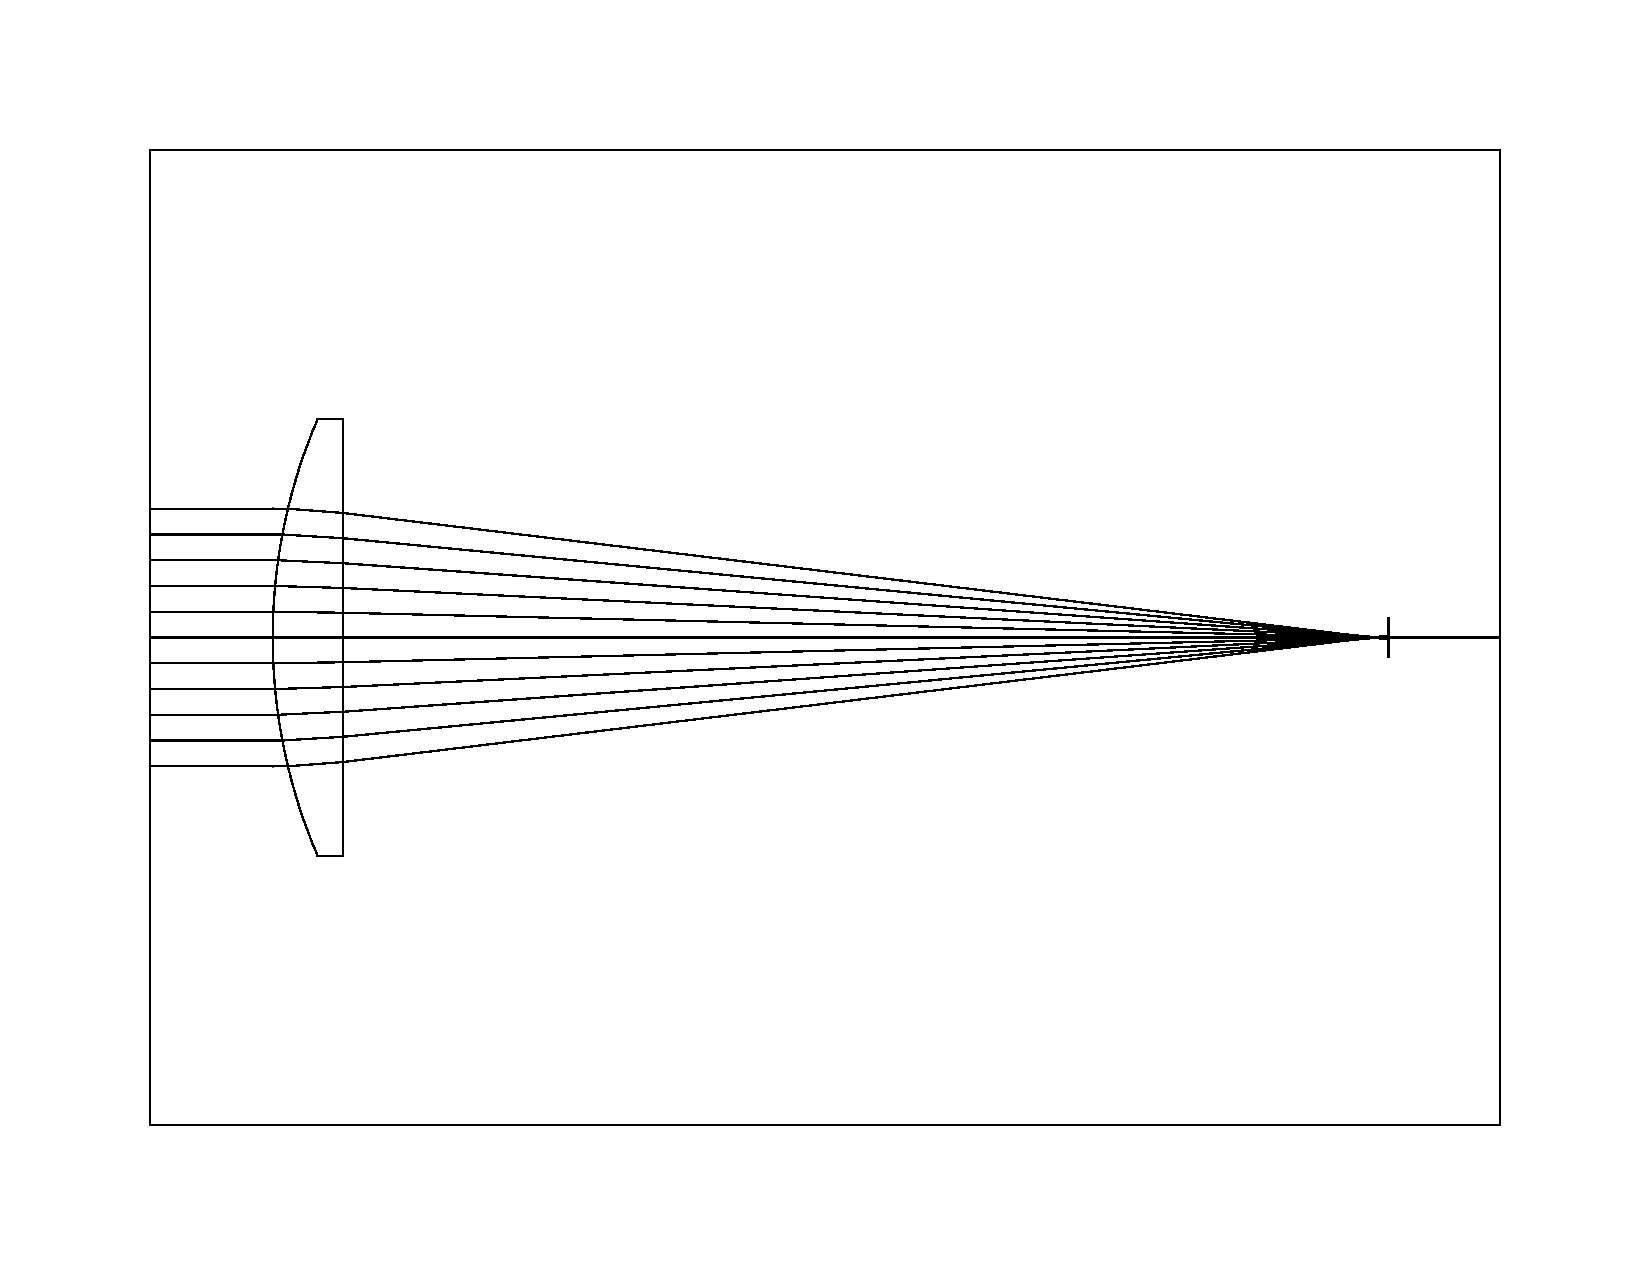
\includegraphics[width=0.5\textwidth]{assets/4 experiments/125lens.pdf}
                \caption{125 mm focal length lens}
            \end{figure}

            \begin{figure}[!ht]
                \centering
                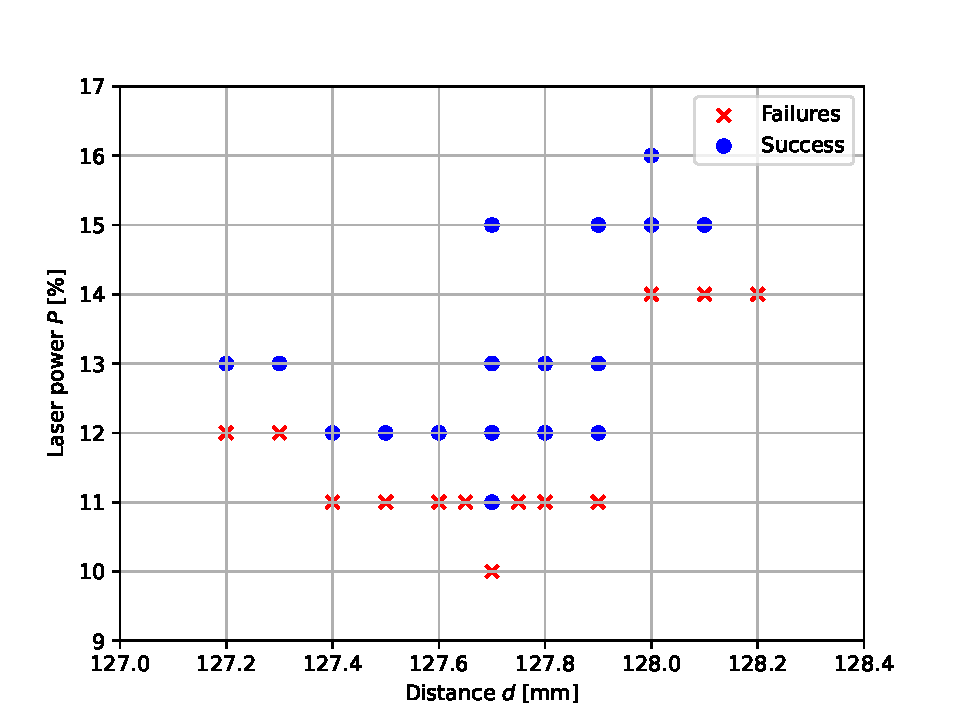
\includegraphics[width=0.75\textwidth]{assets/4 experiments/125mm_focus_threshold.pdf}
                \caption{125 mm focal length lens}
            \end{figure}
            
            Initiation at \qty{11}{\%} was attained once, but it was not possible to replicate this. A tighter focus was necessary to increase initiation reliability.

            % Graph of multi-lens
            \begin{figure}[!ht]
                \centering
                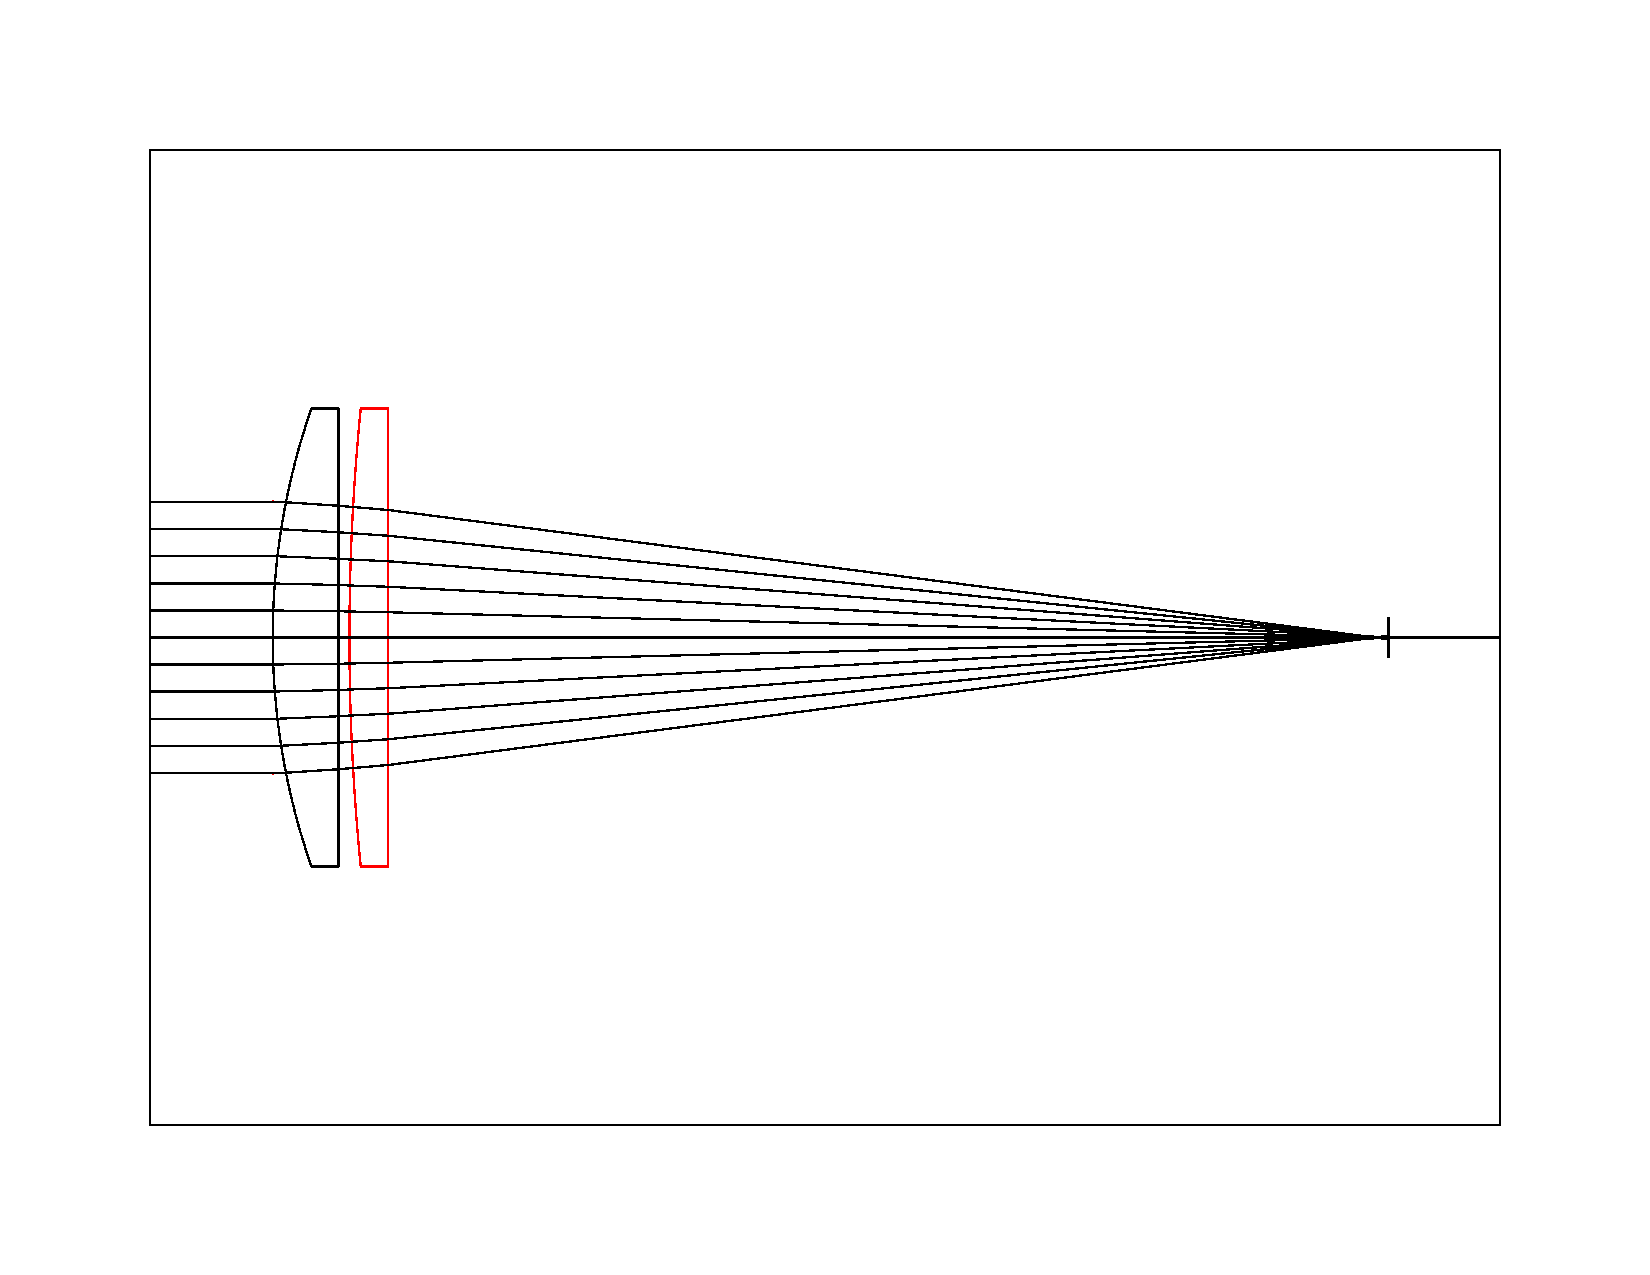
\includegraphics[width=0.5\textwidth]{assets/4 experiments/500 and 150 lenses.pdf}
                \caption{Multi-lens system}
            \end{figure}

            \begin{figure}[!ht]
                \centering
                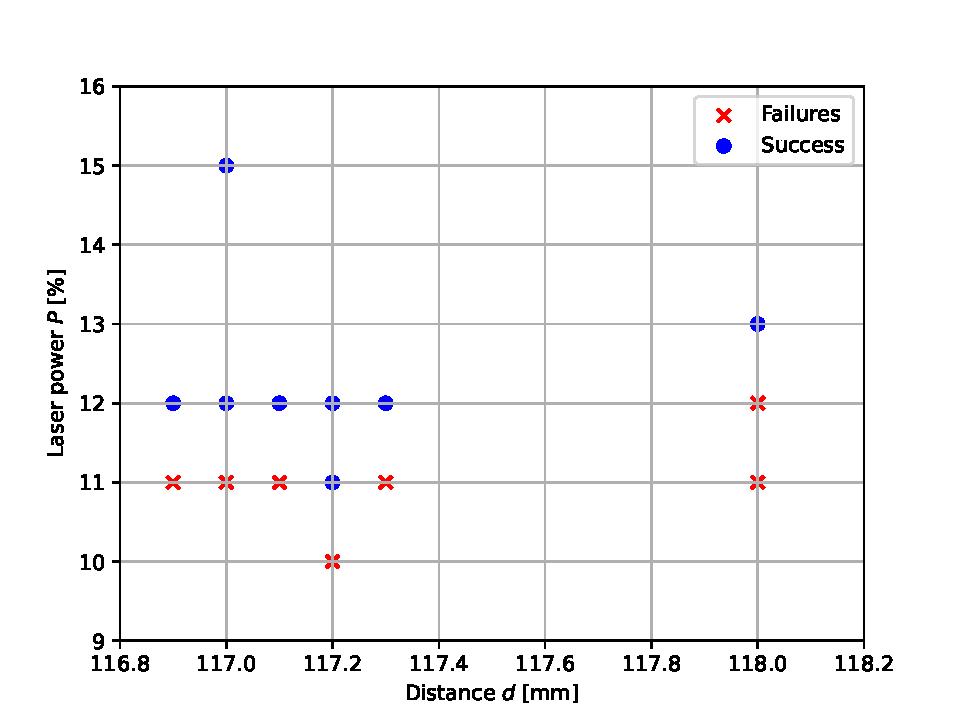
\includegraphics[width=0.75\textwidth]{assets/4 experiments/duallens_focus_threshold.pdf}
                \caption{Multi-lens system}
            \end{figure}

            % Section on power meter reading lower pulsed power at these low power settings, like about 200W

            The completion of these tests validated LSP generation in the CW power regime of the laser. The V2 thruster was then set up to test CW operation with flowing argon.

        \subsection{V2 Bringing the pulsed power down, again}

            To prevent the damage to the thruster seen previously, a rear window mount was manufactured. This allows the laser energy that is not absorbed to pass freely through the apparatus, also enabling power meter measurements. 
            
            % Photo of rear window mount and damaged window

            As can be seen above, the window suffered laser damage after this round of testing. However, this damage proved minor as the window was used to align the laser focus with the spark gap, not to measure power absorption.
            
            The following figure presents the LSP initiation attempts with focus distance, similarly to the graphs presented in \autoref{sec:pulse_power_down_V1}.

            \begin{figure}[!ht]
                \centering
                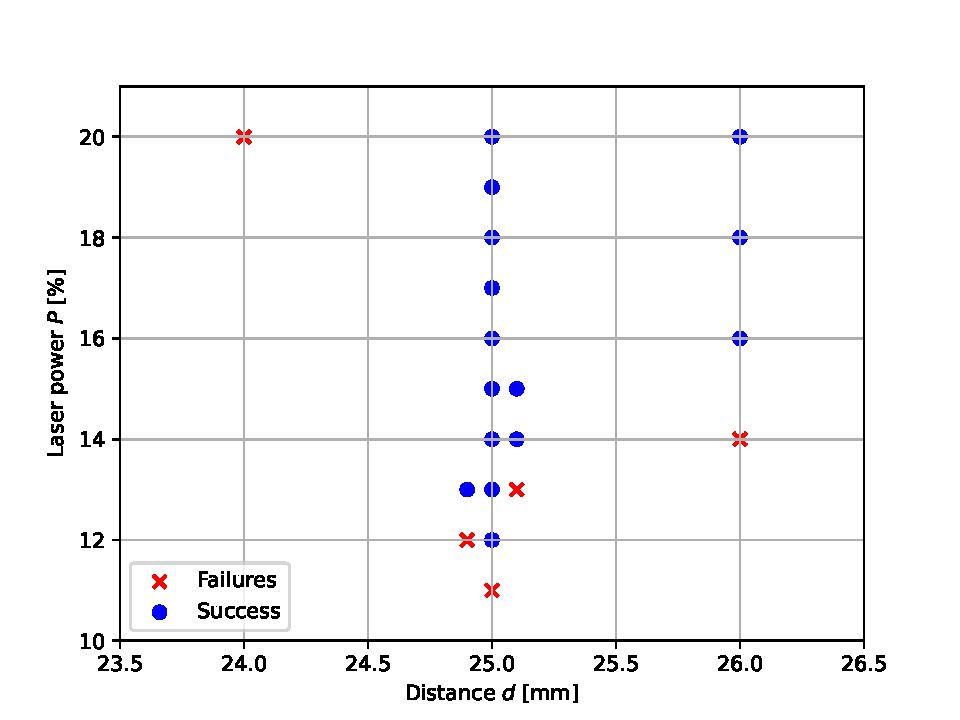
\includegraphics[width=0.75\textwidth]{assets/4 experiments/V2_focus_threshold.pdf}
                \caption{LSP threshold graph for V2}
            \end{figure}

            The real amount of power in the pulsed shots was also measured to validate the \qty{11}{\%} threshold quoted previously. 10 shots each at \qtylist{10; 12}{\%} were measured with the power meter, with statistics compiled by the power meter software (see \autoref{label})

            \begin{table}[!ht]
                \caption{Statistics from the power meter after 10 times \qty{50}{ms} laser shots at \qty{10}{\%} and \qty{12}{\%} power}
                \label{tab:laser shot statistics}
                \begin{tabular}{lll}
                \textbf{Value {[}Unit{]}} & \textbf{10x 50 ms shots at 10\% power} & \textbf{10x 50 ms shots at 12\% power} \\ \hline
                Average value {[}J{]}  & 9.985 & 12.89 \\
                Maximum value {[}J{]}  & 10.2  & 13.3  \\
                Minimum value {[}J{]}  & 9.63  & 12.0  \\
                RMS Stability {[}\%{]} & 1.690 & 2.811 \\
                PTP Stability {[}\%{]} & 5.599 & 10.31 \\
                Average power {[}W{]}  & 0.490 & 1.14  \\
                Std deviation {[}J{]}  & 0.169 & 0.362 \\ \hline
                \end{tabular}
            \end{table}
            
            At 10\% power, an 9.985 J average during \qty{50}{ms} gives an average power of \qty{200}{W}, lower than the expected \qty{300}{W} For \qty{12}{\%}. This revealed a higher power threshold, in terms of percentage, than previously thought. Extrapolating from these measurements, \qty{300}{W} is achieved at \qty{13.5}{\%}. This validated that the

    \section{Static LSP validation}

        \subsection{V1 LSP spark initiation}

            For spark initiation to work reliably, the laser focus and the spark must both be aligned in space and in time.

            % Align in space
            To resolve the spark in the y and z planes (radially) \todo{define this}, the Photron SA5 camera without lens filters was placed in front of the V1 test section, looking in axially. This would be the point of view of the laser beam had it been installed. 

            \begin{figure}[!ht]
                \centering
                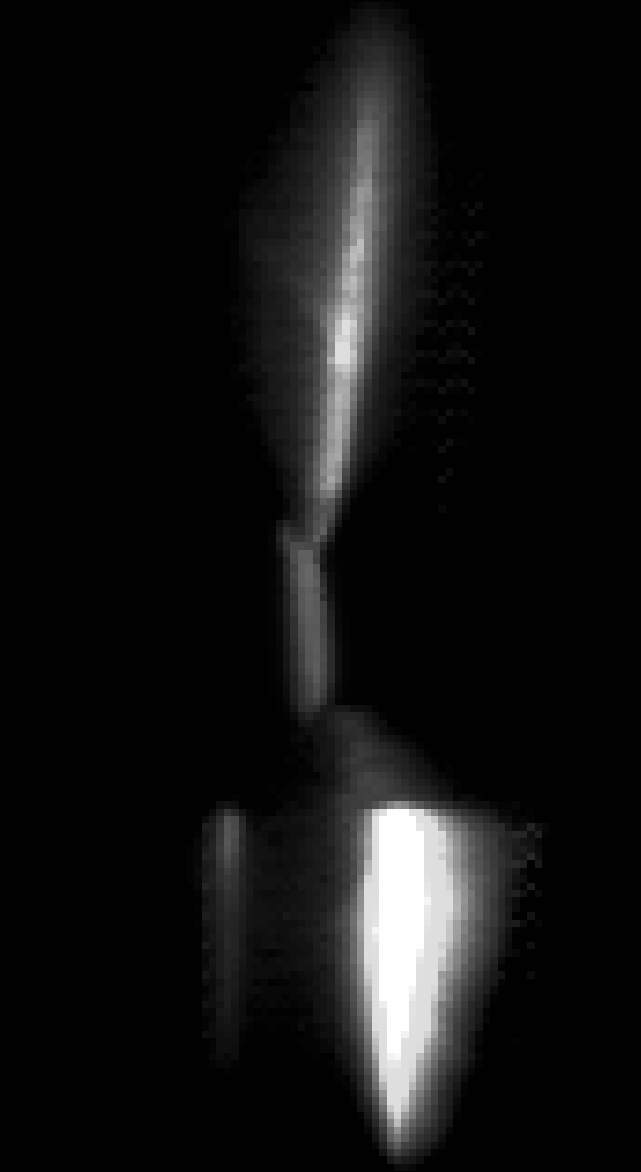
\includegraphics[width=0.25\textwidth]{assets/4 experiments/Composite photo spark.png}
                \caption{Composite photo showing spark between two electrodes. Electrode distance is approximately \qty{1}{mm}}
            \end{figure}
            
            Using the thickness of the electrode as a reference, the spark gap is XX mm and the spark is X mm thick. \todo{measure distance with thickness of electrode}
            The spark is \todo{measure this too} X mm thick.
            
            % Link between the two
            As the spark was recorded by the high speed camera, timing data was also collected for the spark.
            
            % Align in time
            To align the laser focus to the spark in time, the infrared laser being invisible to the camera, the beam was focused on one of the electrodes at low power. This caused the steel to glow white-hot when the laser was on. The following timings were determined by this investigation: \todo{reword this}

            \begin{figure}
                \centering
                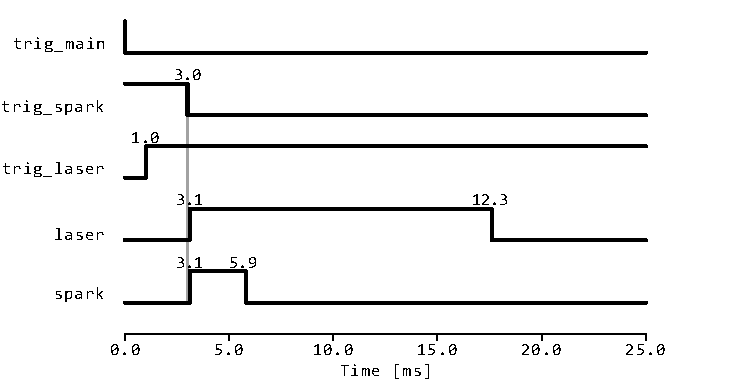
\includegraphics[width=\textwidth]{assets/4 experiments/timings.pdf}
                \caption{Signal timing diagram. The \textit{trig} prefix denotes triggering signals. The component is active when the line is high. Timings in \unit{ms} are also indicated on the figure.}
            \end{figure}

            \begin{figure}[h]
    \centering
    \begin{subfigure}[t]{0.3\textwidth}
        \centering
        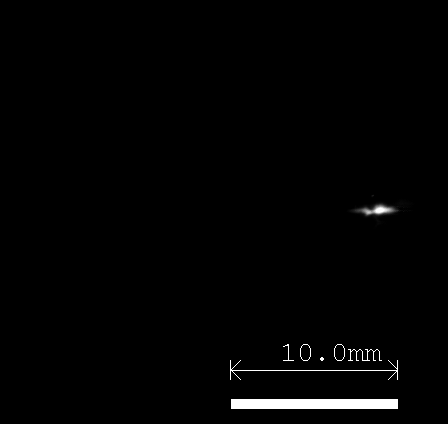
\includegraphics[width=\textwidth]{assets/4 experiments/V1 Spark Ignition Frames/LSP142_SPRK15_Fr32.bmp}
        \caption{\qty{3.2}{ms}}
        %\label{fig:V1_ignition_frames_16}
    \end{subfigure}
    \hfill
    \begin{subfigure}[t]{0.3\textwidth}
        \centering
        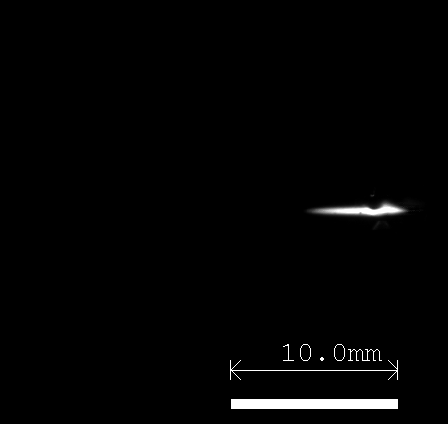
\includegraphics[width=\textwidth]{assets/4 experiments/V1 Spark Ignition Frames/LSP142_SPRK15_Fr33.bmp}
        \caption{\qty{3.3}{ms}}
        %\label{fig:ignition_frames_17}
    \end{subfigure}
    \hfill
    \begin{subfigure}[t]{0.3\textwidth}
        \centering
        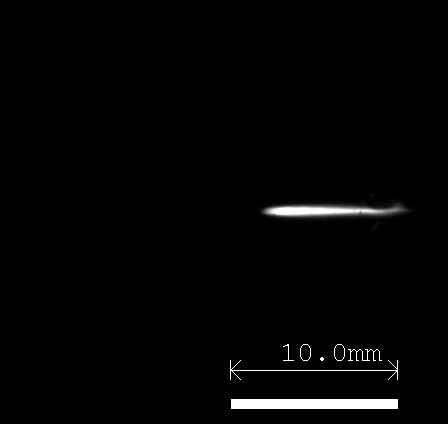
\includegraphics[width=\textwidth]{assets/4 experiments/V1 Spark Ignition Frames/LSP142_SPRK15_Fr35.bmp}
        \caption{\qty{3.5}{ms}}
        %\label{fig:ignition_frames_18}
    \end{subfigure}
    \begin{subfigure}[t]{0.3\textwidth}
        \centering
        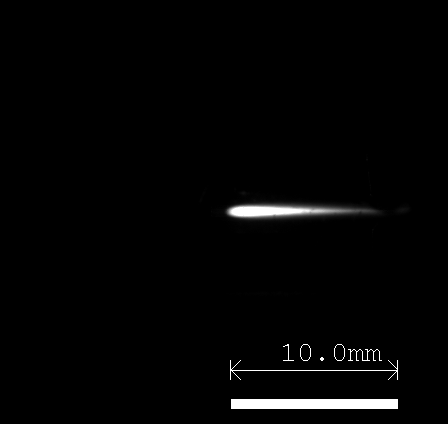
\includegraphics[width=\textwidth]{assets/4 experiments/V1 Spark Ignition Frames/LSP142_SPRK15_Fr38.bmp}
        \caption{\qty{3.8}{ms}}
        %\label{fig:ignition_frames_19}
    \end{subfigure}
    \hfill
    \begin{subfigure}[t]{0.3\textwidth}
        \centering
        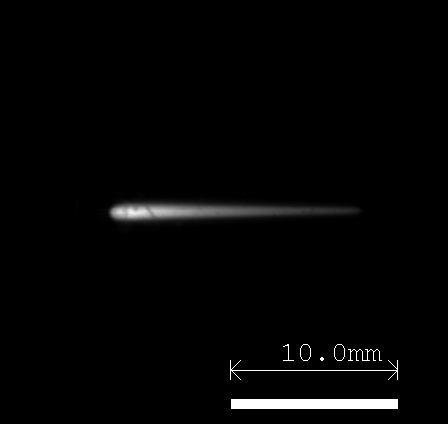
\includegraphics[width=\textwidth]{assets/4 experiments/V1 Spark Ignition Frames/LSP142_SPRK15_Fr69.bmp}
        \caption{\qty{6.9}{ms}}
        %\label{fig:ignition_frames_20}
    \end{subfigure}
    \hfill
    \begin{subfigure}[t]{0.3\textwidth}
        \centering
        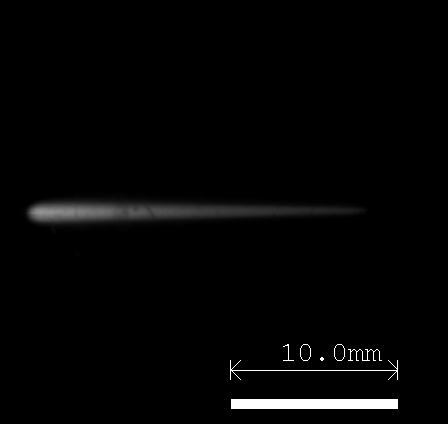
\includegraphics[width=\textwidth]{assets/4 experiments/V1 Spark Ignition Frames/LSP142_SPRK15_Fr130.bmp}
        \caption{\qty{13.0}{ms}}
        %\label{fig:ignition_frames_21}
    \end{subfigure}
    \caption{LSP spark initiation: \qty{3080}{W}, \qty{20}{bar}. \shotsettings{LSP142\_SPRK15}{0.1?? CHANGE}{22}{2048}}
    \label{fig:V1_spark_initiation_frames}
\end{figure}

            \missingfigure{pressure rise with V1 LSP spark initiation}

            \subsection{\ce{NO2} seeding}

            \todo{Comment from Prof. Higgins: If you want to present the NO2 work, you'll need to: Explain attenuation/absorption coefficient as it appears in Beer-Lambert law and how this defines the length scale over which absorption occurs. Explain how absorption coefficient is derived from the cross section of the molecule, which will involve using the  HITRAN database, etc. It is not acceptable to just say "we added NO2" and reference it off to some paper.}
            
            As the plasma emits in the ultraviolet (UV) range, it is necessary to seed with a gas that absorbs UV but not the infrared (IR) laser. \textcite{khanGasDetectionUsing2019} shows that \ce{NO2} and \ce{SO2} are two candidates. \ce{NO2} was first used as it was easy to produce in-house in significant quantities. The V1 system was set up with a vacuum pump connected to an outside air exhaust to safely vent the \ce{NO2} gas. The pump was also used to bring the pressure in the test section down to vacuum (how much?) before introducing gas.

            %[Add absorption spectrum of NO2 from Gas Detection Using Portable Deep-UV Absorption Spectrophotometry: A Review or other place]

            Control LSP shots were undertaken in pure argon. Next, 0.55 bar of \ce{NO2}, or 200 mL at STP, were introduced into the chamber. It was then pressurized with argon to 20 bar. With the spark active, LSPs were consistently generated in the seeded atmosphere and their pressure trace from the PCB transducer was recorded with the oscilloscope. This pressure rise was approximately double the one seen in pure argon; see \autoref{fig:NO2_shots_analysis}.

            The next series of LSP shots was conducted with 0.24 bar (\qty{85}{ml} at STP) of \ce{NO2} and filled to 20.2 bar of argon. Again, higher pressure rises were observed, but slightly less than the \qty{0.55}{bar} shots. The chamber was finally half evacuated to 10.17 bar and then filled back to \qty{20.15}{bar}. This should bring the partial pressure of \ce{NO2} to \qty{0.12}{bar}. Again, LSPs were consistent, with a higher pressure rise than pure argon, but less than the higher concentration \ce{NO2} shots.

            \begin{figure}[!ht]
                \centering
                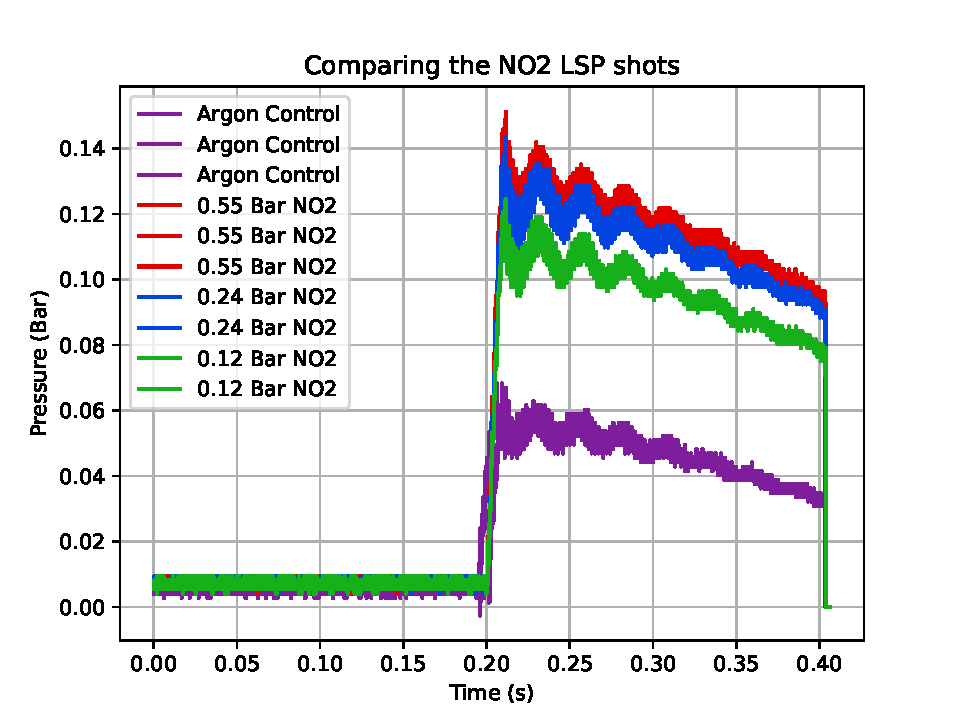
\includegraphics[width=0.75\textwidth]{assets/4 experiments/NO2_shots_analysis.pdf}
                \caption{Comparing \ce{NO2} LSP shots to pure argon LSP shots}
                \label{fig:NO2_shots_analysis}
            \end{figure}

            Indeed, with as low as (0.5\%?) of \ce{NO2} mixed with argon, nearly double the pressure rise is observed. This indicates that the working gas is absorbing twice the energy from the plasma. As the \ce{NO2} fraction is increased, there are diminishing returns to the pressure rise. This is encouraging, as not much \ce{NO2} is needed to have a great impact on the energy absorption.

        

        \subsection{V2 LSP spark initiation and QCW LSP}

            % Methodology

            As timing of the spark and laser focus was kept the same as the previous section (ref), only the methodology of spatial alignement will be covered here.

            % Methodology of V2 spark initiation: moving the test section back and forth on the rail gave a reliable way to align spatially . Then 2 figures: wide fov and tight fov, stills from the alignment video I took on the power meter

            The power meter was used as a screen to align the laser focus. By moving the V2 test section back and forth on the thrust stand rail, the field of view (FOV) of the shadows projected on the power meter can be modified (see \autoref{fig:FOV}). 
            
            \begin{figure}[!ht]
                \centering
                \begin{subfigure}[t]{0.45\textwidth}
                    \centering
                    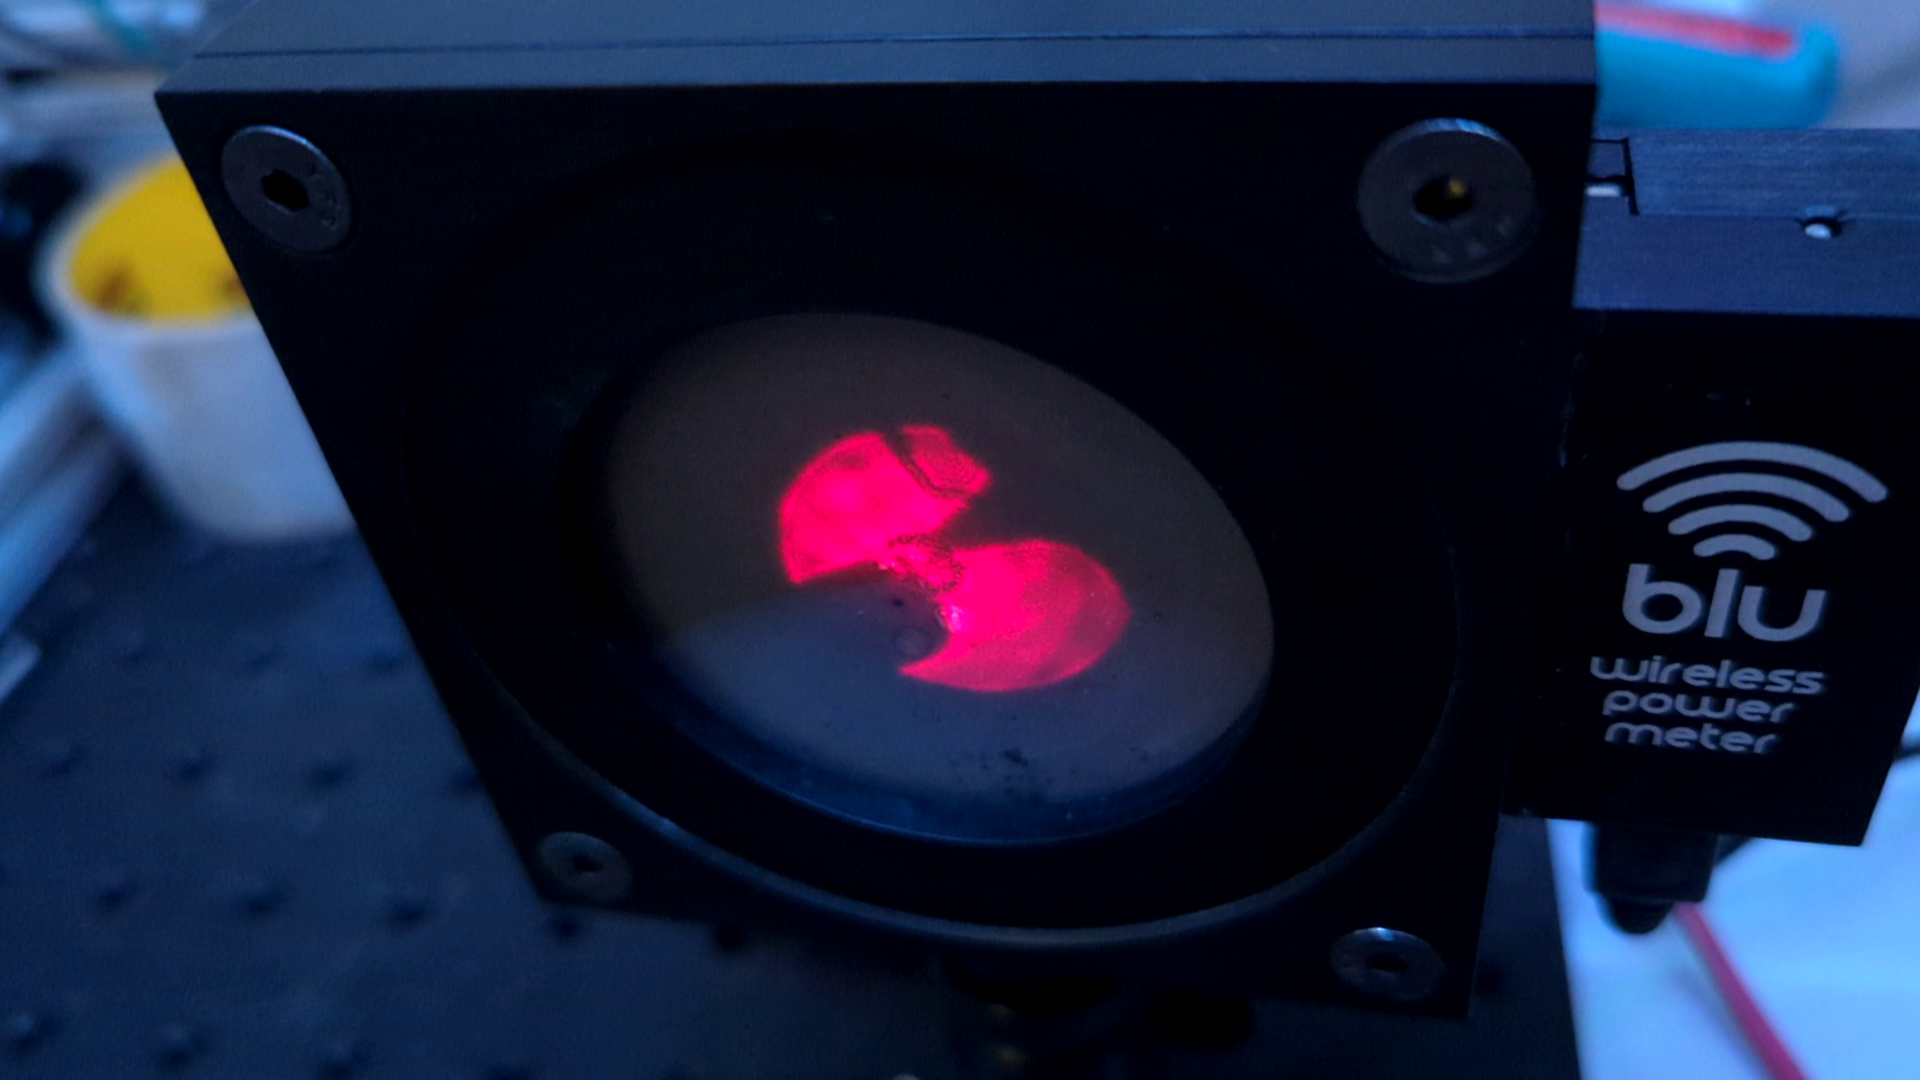
\includegraphics[width=\textwidth]{assets/4 experiments/V2 alignment 1.png}
                    \caption{V2 alignment, zoomed out}
                \end{subfigure}
                \hfill
                \begin{subfigure}[t]{0.45\textwidth}
                    \centering
                    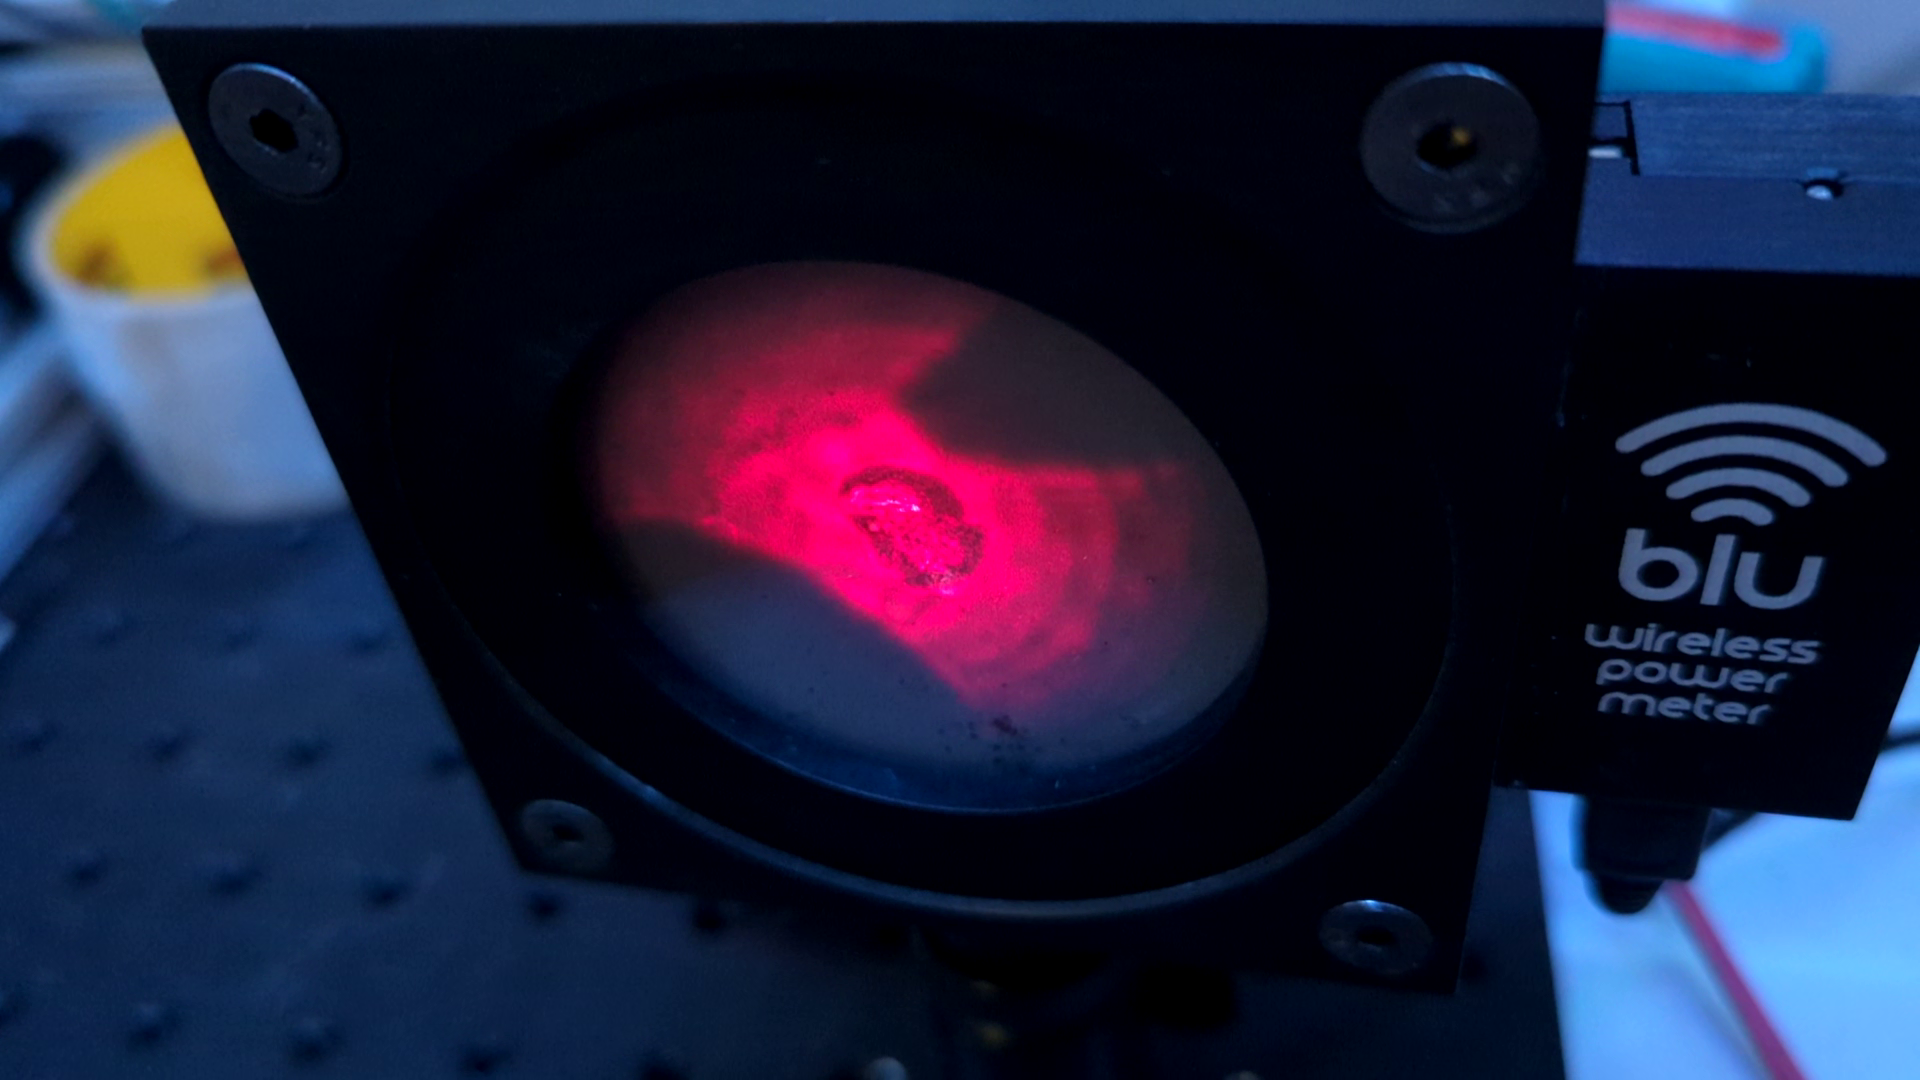
\includegraphics[width=\textwidth]{assets/4 experiments/V2 alignment 2.png}
                    \caption{V2 alignment, zoomed in}
                \end{subfigure}
                \caption{2 FOVs of laser light on powermeter. The abberation at the center of the red light is due to laser damage to the window.}
                \label{fig:FOV}
            \end{figure}



            The laser can then be moved so that the area where the visible alignment laser is brightest matches the center of the electrodes' shadow. 
            % Discussion: could do this when V2 is open (without putting flat back plate and before pressurizing) however, electrodes move a bit (approx 1mm) when pressurized so alignement is not perfect. Also, if alignement is not satisfactory the first time, the test section must be depressurized and the backplate taken off. The laser is realigned, back plate sealed back on (8 M2 screws to tighten) and test section must be purged again. THIS TAKES TOO LONG! It is easier to align with a rear window (final static LSP configuration), as the test section can be pressurized while the laser is being aligned, and the alignment can be changed without taking the window mount off.

            

            % Stills of first High-speed LSP video, showing expansion of LSP wave like in V1

            As these are at an angle and we are looking at the reflection of the LSP, no LSP velocity measurements can be made.

            With the Photron SA5 looking into the thruster from the front, LSP initiation was confirmed in V2. \todo{complete V2 initiation section, add photos, remove one of these 2 sentences}

            \begin{figure}[!ht]
                \centering
                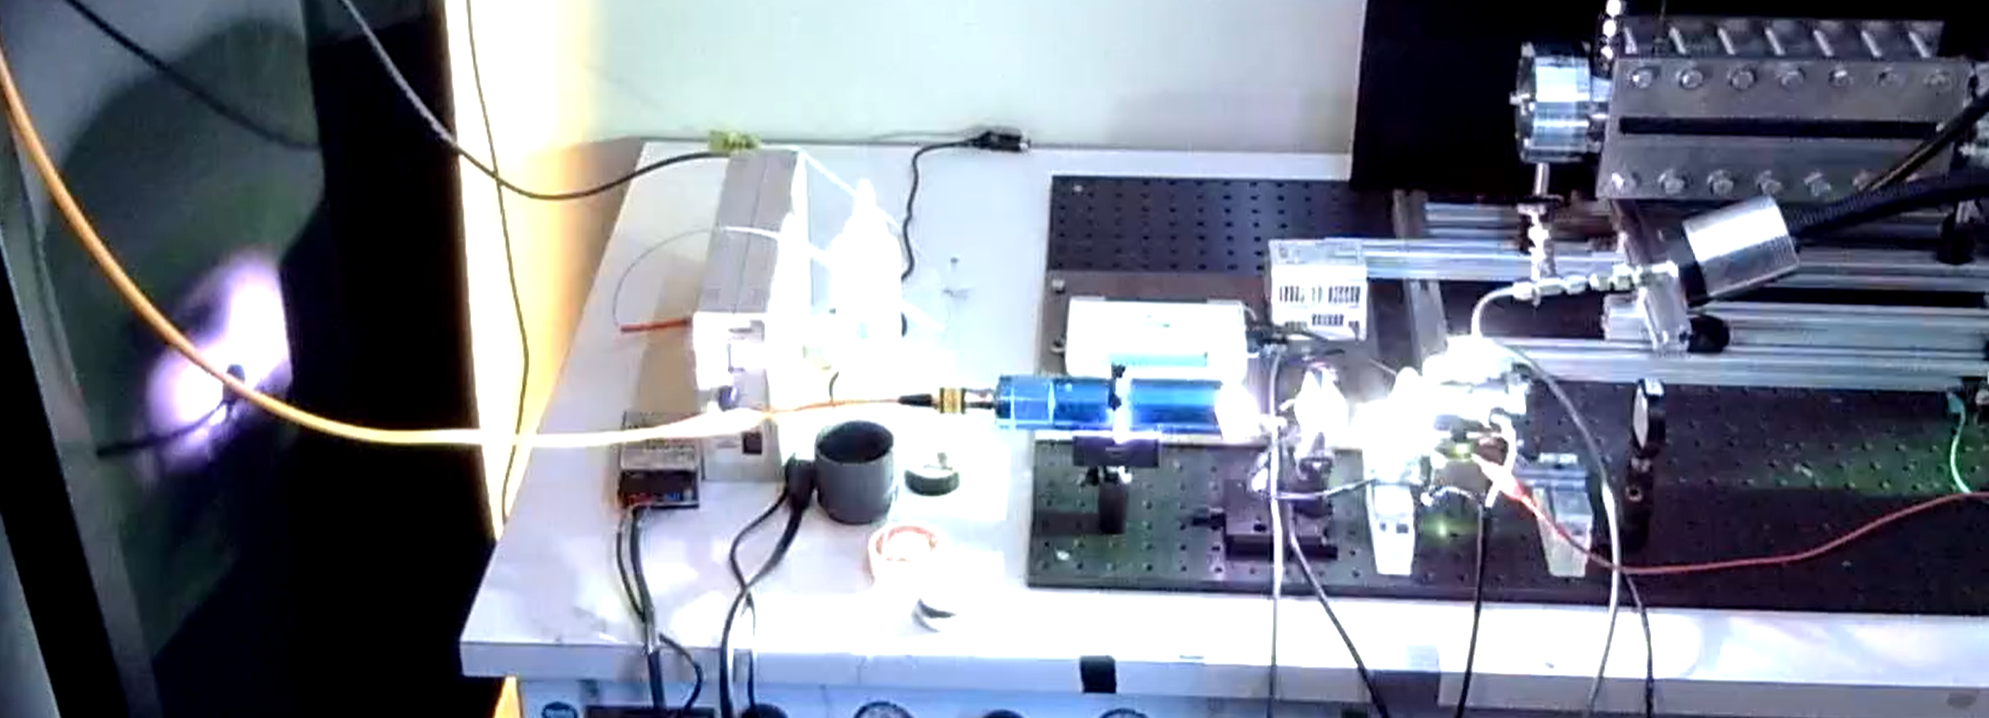
\includegraphics[width=0.5\textwidth]{assets/4 experiments/holy jesus look at this.png}
                \caption{ PLACEHOLDER! 100\% power (quantify) QCW LSP shot. Note the bright plasma emission axially upstream of V2 on the laser safety curtain.}
            \end{figure}

            \todo{placeholder picture}



        \subsection{V2 CW LSP}

            A \qty{100}{\%} power CW shot was then attempted at \qty{20}{bar} argon. 

            [photo of laser on, Spark/LSP initiation, LSP constant, laser off (LSP dying down)]

            \missingfigure{frames of high speed camera to show growth of plasma in V2}

            %\begin{figure}[h]
    \centering
    \begin{subfigure}[t]{0.3\textwidth}
        \centering
        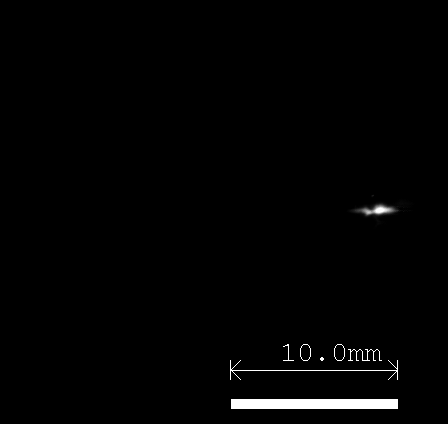
\includegraphics[width=\textwidth]{assets/4 experiments/V1 Spark Ignition Frames/LSP142_SPRK15_Fr32.bmp}
        \caption{\qty{3.2}{ms}}
        %\label{fig:V1_ignition_frames_16}
    \end{subfigure}
    \hfill
    \begin{subfigure}[t]{0.3\textwidth}
        \centering
        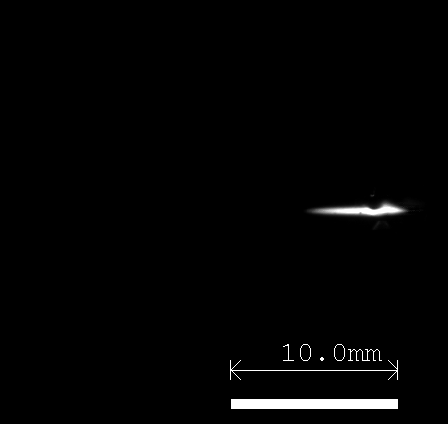
\includegraphics[width=\textwidth]{assets/4 experiments/V1 Spark Ignition Frames/LSP142_SPRK15_Fr33.bmp}
        \caption{\qty{3.3}{ms}}
        %\label{fig:ignition_frames_17}
    \end{subfigure}
    \hfill
    \begin{subfigure}[t]{0.3\textwidth}
        \centering
        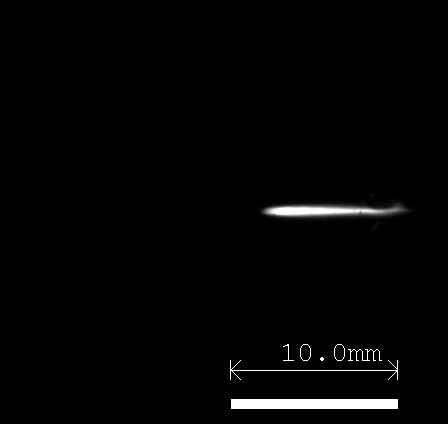
\includegraphics[width=\textwidth]{assets/4 experiments/V1 Spark Ignition Frames/LSP142_SPRK15_Fr35.bmp}
        \caption{\qty{3.5}{ms}}
        %\label{fig:ignition_frames_18}
    \end{subfigure}
    \begin{subfigure}[t]{0.3\textwidth}
        \centering
        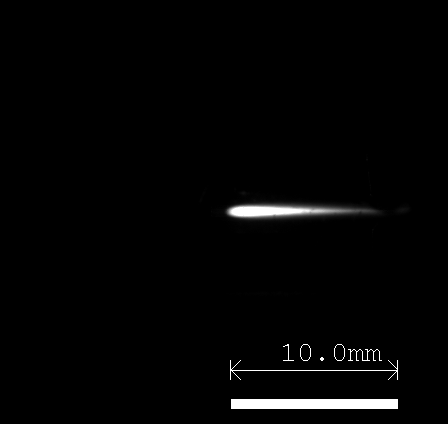
\includegraphics[width=\textwidth]{assets/4 experiments/V1 Spark Ignition Frames/LSP142_SPRK15_Fr38.bmp}
        \caption{\qty{3.8}{ms}}
        %\label{fig:ignition_frames_19}
    \end{subfigure}
    \hfill
    \begin{subfigure}[t]{0.3\textwidth}
        \centering
        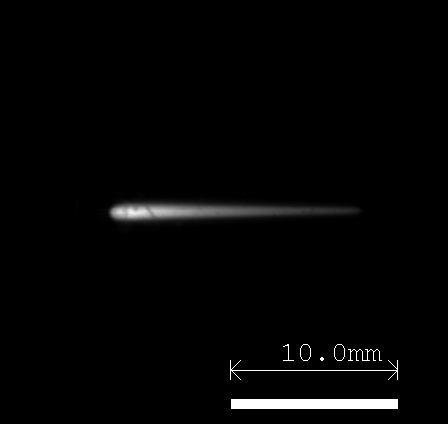
\includegraphics[width=\textwidth]{assets/4 experiments/V1 Spark Ignition Frames/LSP142_SPRK15_Fr69.bmp}
        \caption{\qty{6.9}{ms}}
        %\label{fig:ignition_frames_20}
    \end{subfigure}
    \hfill
    \begin{subfigure}[t]{0.3\textwidth}
        \centering
        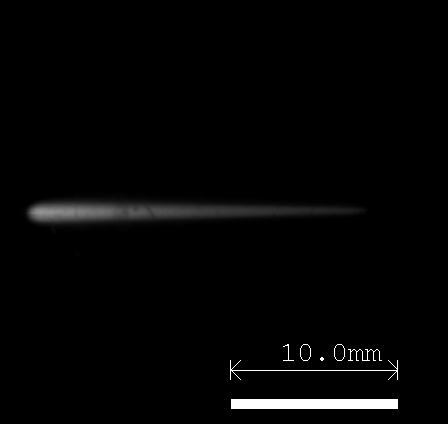
\includegraphics[width=\textwidth]{assets/4 experiments/V1 Spark Ignition Frames/LSP142_SPRK15_Fr130.bmp}
        \caption{\qty{13.0}{ms}}
        %\label{fig:ignition_frames_21}
    \end{subfigure}
    \caption{LSP spark initiation: \qty{3080}{W}, \qty{20}{bar}. \shotsettings{LSP142\_SPRK15}{0.1?? CHANGE}{22}{2048}}
    \label{fig:V1_spark_initiation_frames}
\end{figure}

            First the laser is turned on. A flash marks the spark initiation and instant LSP initiation. The laser was kept running for about a second before it is turned off.

            Observation of the high speed camera footage, recorded at 10000 frames per second, showed the CW LSP starting at frame 32 (\qty{3.2}{ms}) and ending at frame 883 (\qty{88.3}{ms}), lasting \qty{85.1}{ms}. This represents a 1.7 times longer lifetime than the maximum QCW pulse length of \qty{50}{ms} at this power.


            \begin{figure}[!ht]
                \centering
                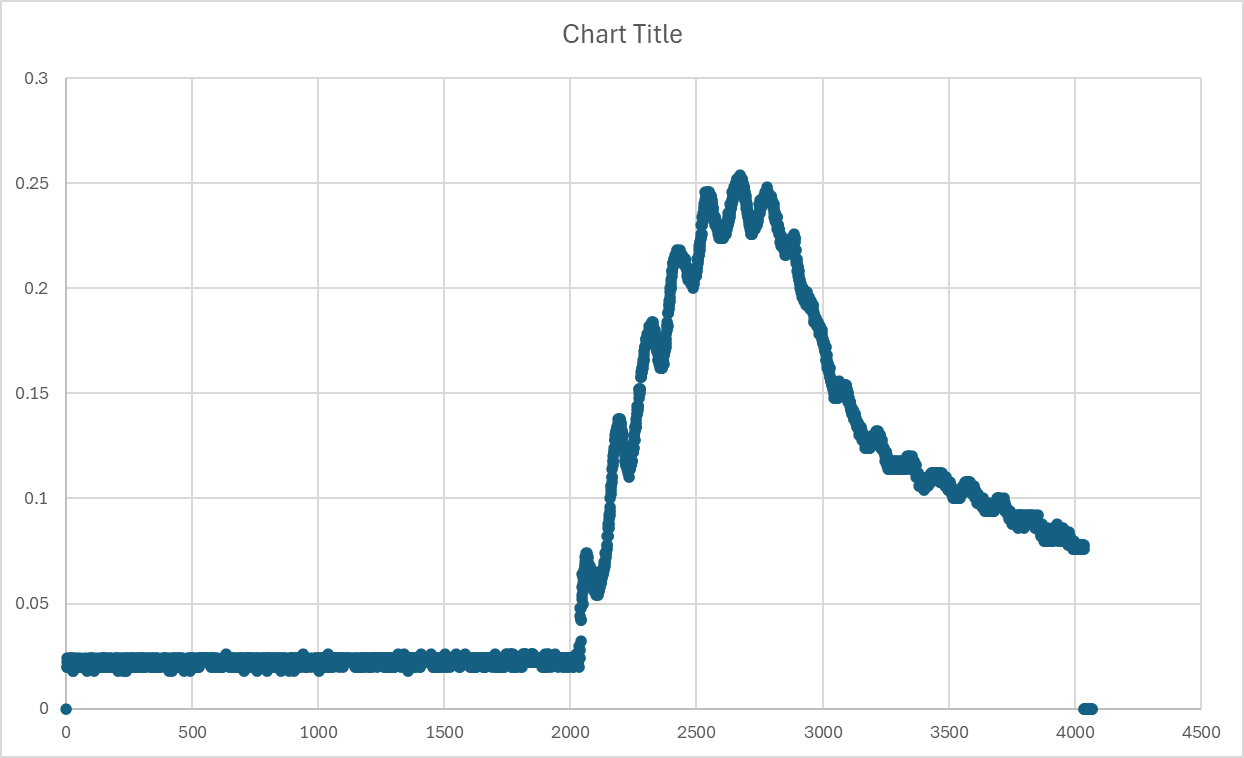
\includegraphics[width=0.5\textwidth]{assets/4 experiments/CW pressure rise.png}
                \caption{Pressure rise with PCB transducer}
            \end{figure}

            This graph shows the pressure rise recorded by the PCB transducer connected to the oscilloscope. This was the first CW LSP generated in the lab. \todo{make better graph} Minimal damage to the window was noticed after this test, suggesting that the LSP absorbed a portion of the laser energy.

        \subsection{CW power measurement}

            Wanted to see where exactly the pulsed power threshold was. For this, needed a max CW power measurement to compare against. 
    
            Tried to measure max CW power through two lenses, without the V2 apparatus. The two lenses were rated for this flux, but the 500 mm focal length lens shattered after about \qty{50}{s} of CW lasing. The leading hypothesis is that as the lens' temperature increased, it expanded, shattering it
    
            [graph of laser power that broke lens]
    
            \begin{figure}[!ht]
                \centering
                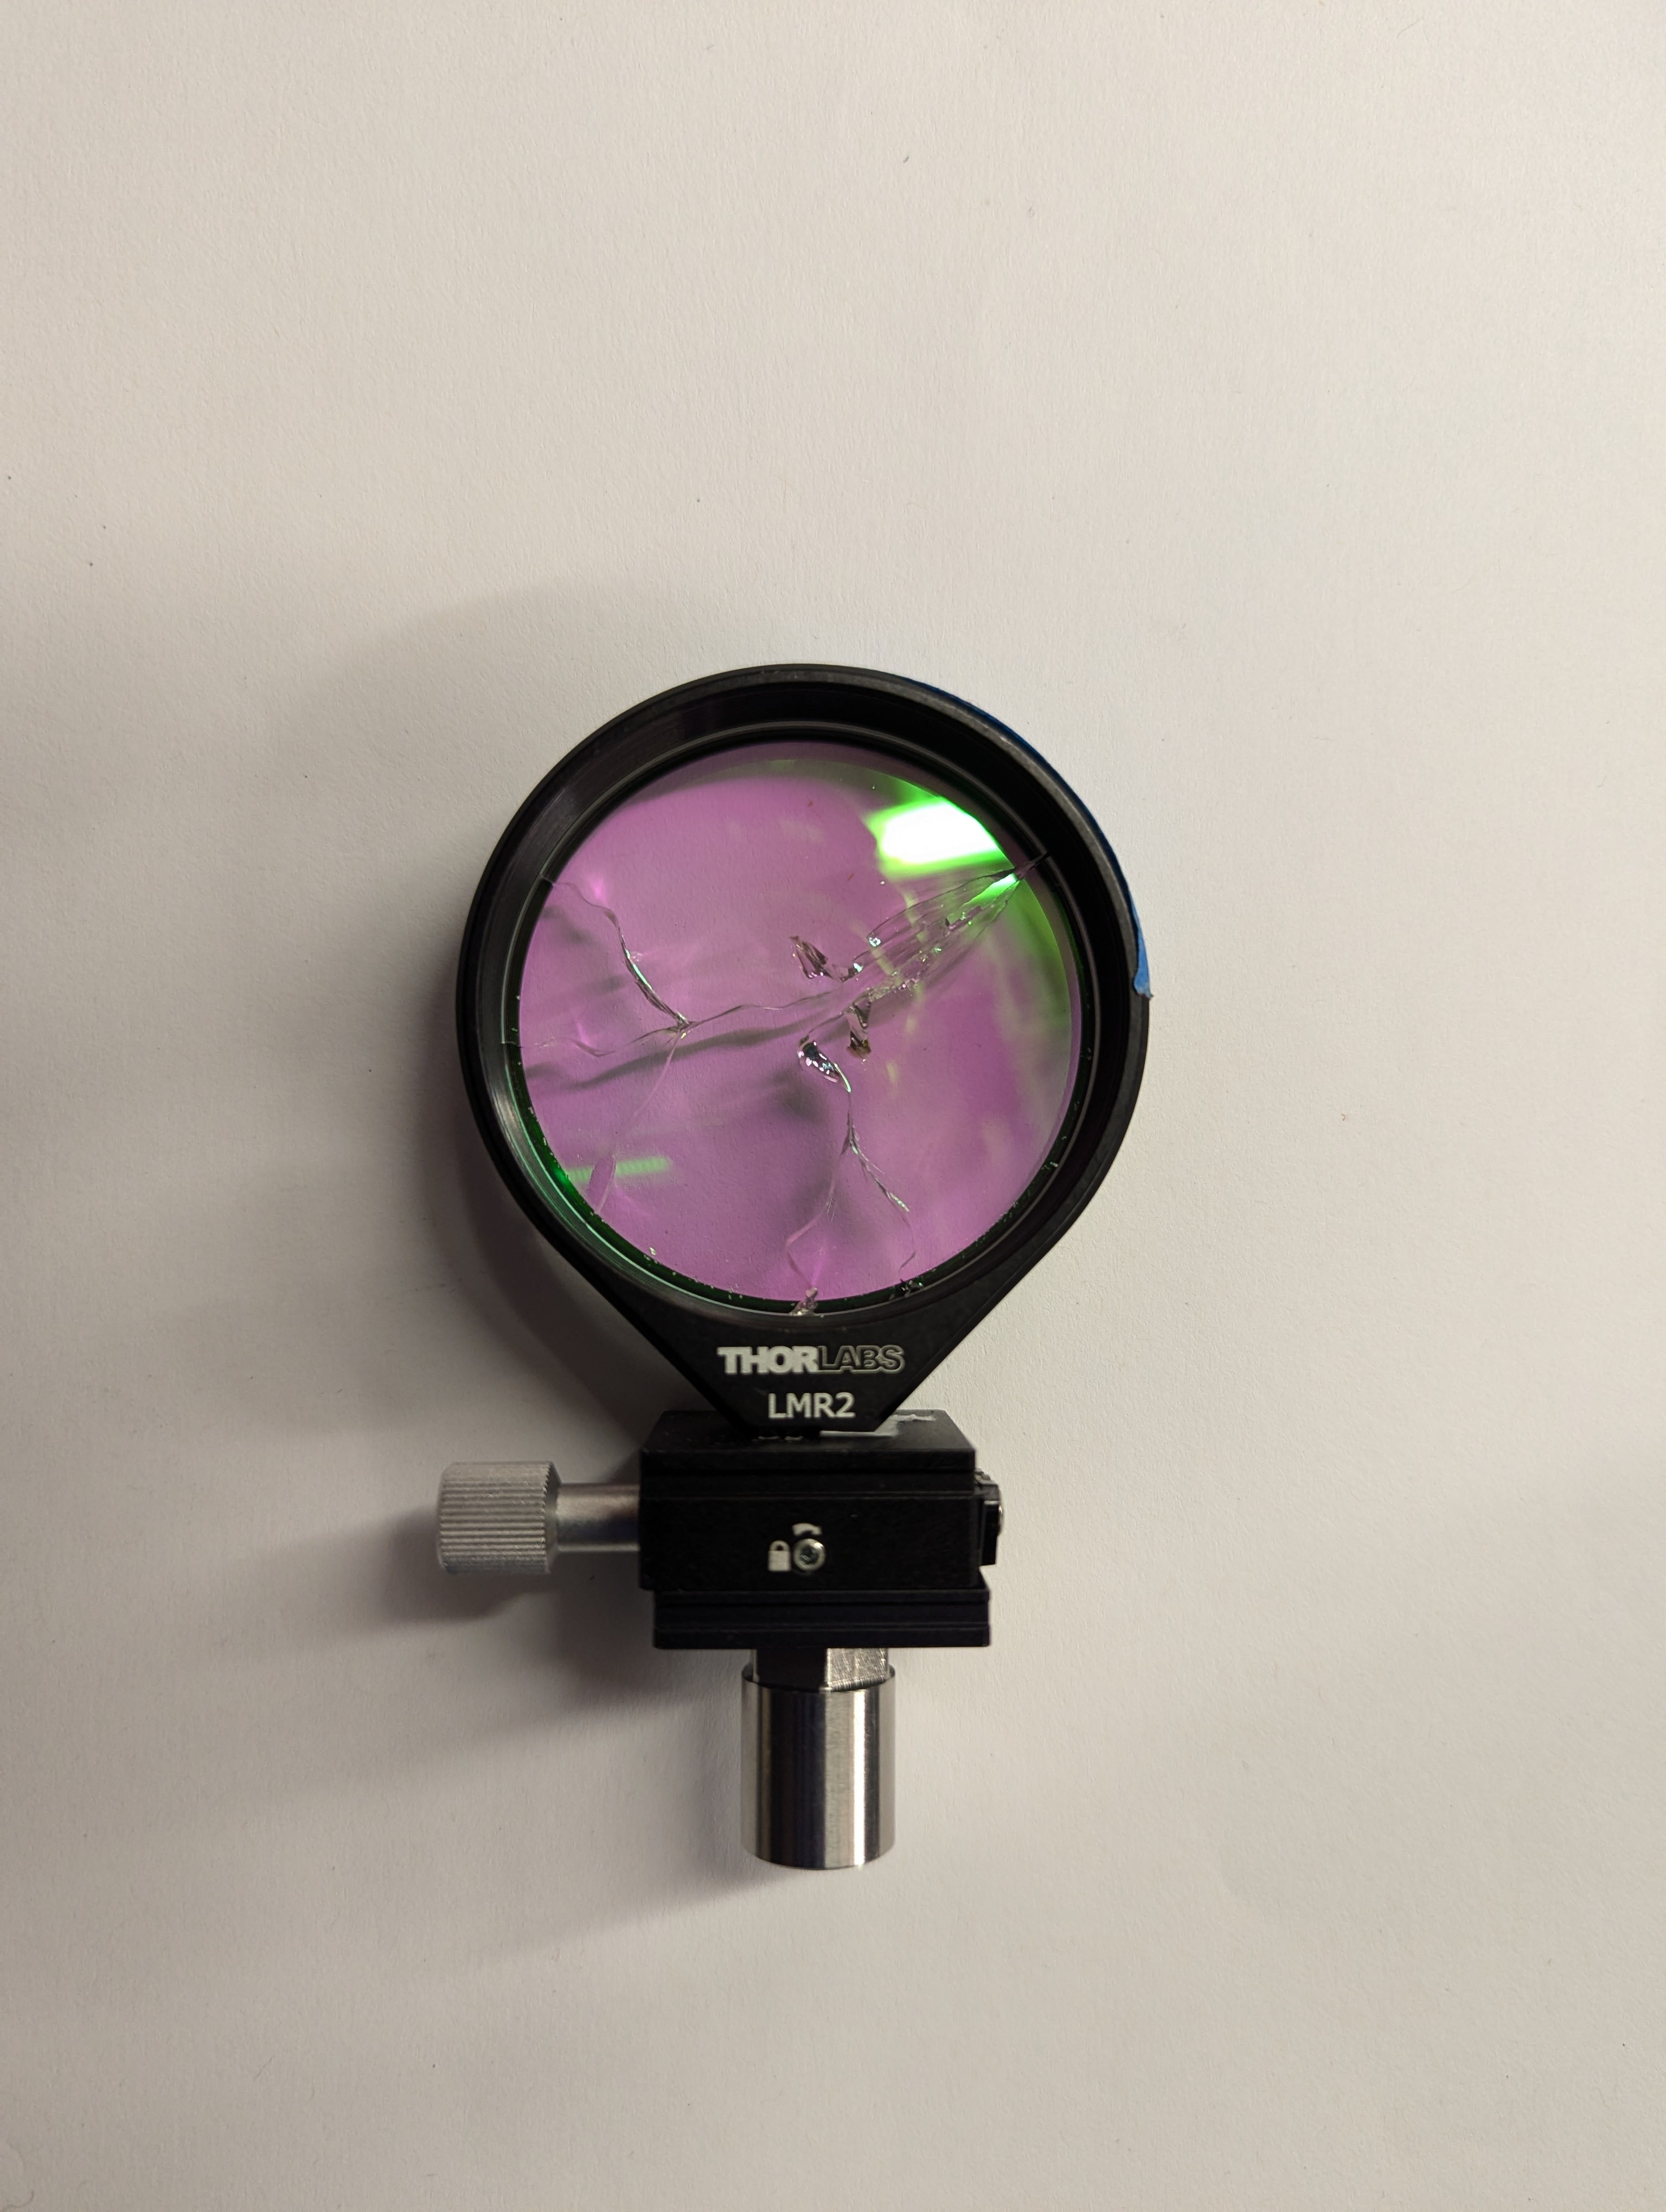
\includegraphics[width=0.25\textwidth]{assets/4 experiments/Shattered 500 mm lens.jpg}
                \caption{Shattered \qty{500}{mm} focal length lens}
            \end{figure}
    
            This test showed a \qty{316}{W} (?) max CW power.
    
            Therefore, future CW tests will have to stay under this maximum time period, unless a lens cooling system is implemented. This could be as simple as a fan blowing cool air onto the lens.

        \subsection{Summary of results}

            \begin{table}[!ht]
                \centering
                \caption{Summary of the static LSP validation campaign}
                \label{tab:validation}
                \begin{tabular}{@{}lll@{}}
                \toprule
                Validation Question               & Yes & No \\ \midrule
                Is LSP spark initiation possible? & X   &    \\
                Is QCW LSP possible in V2?        & X   &    \\
                Is CW LSP possible in V2?         & X   &   
                \end{tabular}
            \end{table}


    \section{Cold flow thruster characterisation}

        \subsection{Cold flow thrust tests}

            Cold flow tests (laser off) were completed to give a baseline measurement of thrust before eventual hot fire tests (laser on), and to validate the functioning of all data acquisition systems. Refer to appendix for Omega pressure sensor calibration \todo{Add pressure sensor calibration in appendix}.

            For thrust tests, pressure and thrust were recorded. \autoref{fig:20bar cold flow} shows a typical thrust and pressure curve for a chamber pressure of \qty{20}{bar}. Note that the thrust measurement does not return to the same value it was at initially.

            \begin{figure}[!ht]
                \centering
                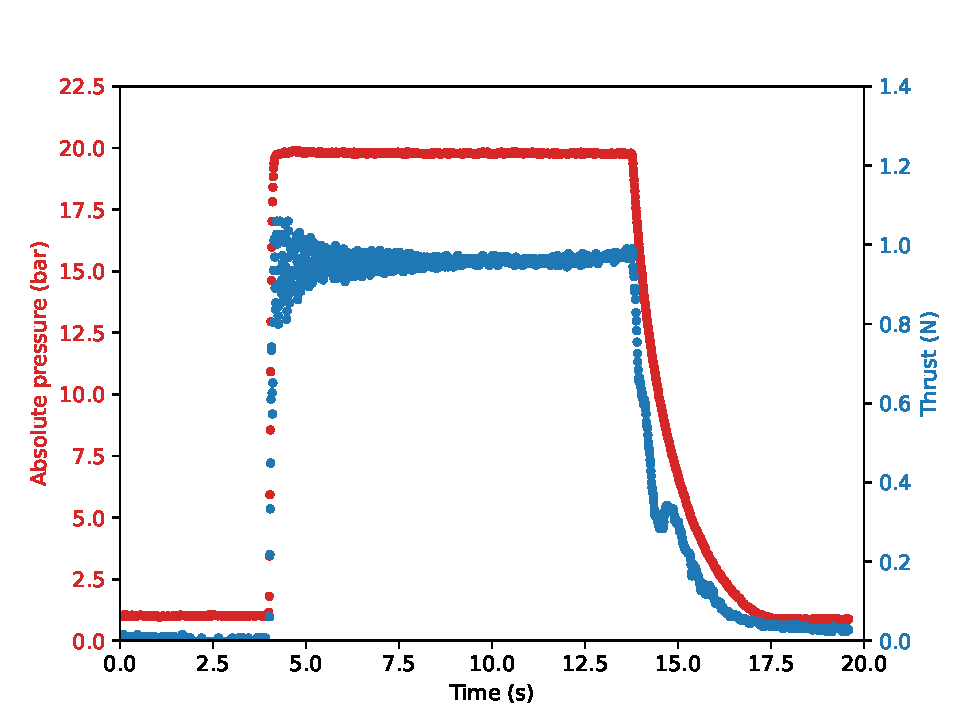
\includegraphics[width=0.75\textwidth]{assets/4 experiments/Example thrust 20 bar.pdf}
                \caption{Typical cold flow pressure and thrust curves for 20 bar chamber pressure}
                \label{fig:20bar cold flow}
            \end{figure}

            Next, cold flow thrust tests were completed at chamber pressures from \qtyrange{5}{35}{bar}. 5 were done for each nominal pressure in steps of \qty{5}{bar}, for a total of 35 tests \todo{cold flow thrust vs pressure relation graph needs Siera's 35 points}. A linear curve fit of the experimental results is presented in \autoref{fig:coldflow pressure-thrust}.

            \begin{figure}[!ht]
                \centering
                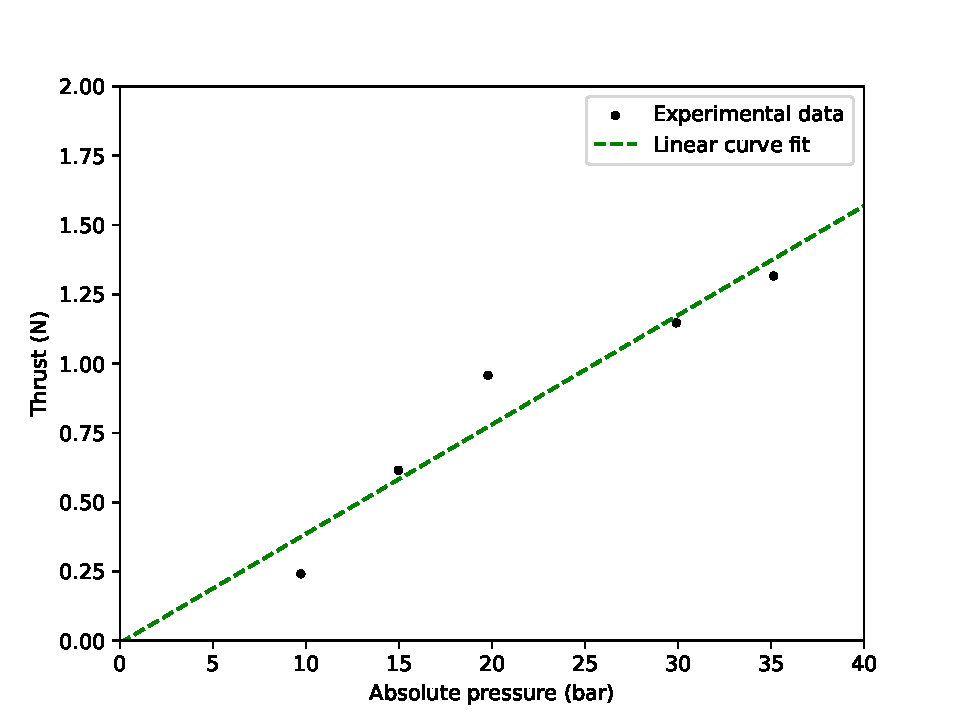
\includegraphics[width=0.75\textwidth]{assets/4 experiments/pressure-thrust graph.pdf}
                \caption{Absolute pressure versus thrust with 35 experimental points and curve fit of pressure-thrust relation}
                \label{fig:coldflow pressure-thrust}
            \end{figure}

            The empirical relation of thrust versus pressure is given by... \todo{insert relation here}.

        \subsection{Thruster nozzle effective sonic area $A^*$}

            To determine mass flow, \todo{Explain how we want to measure mass flow lol}
        
            To characterise the effective sonic area, $A^*$, of the thruster nozzle, a choked orifice blow-down test was undertaken based upon the theory in \textcite{saadCompressibleFluidFlow}. V2 in flowing configuration was pressurized to \qty{20}{bar} of argon. The argon flow was then closed. The pressure curve was recorded by the Omega \todo{part number} transducer.

            \todo{In discussion, talk about the issue of nozzle A* being smaller with 5 papers from June 4th on slack.}

            The internal volume of the V2 thruster in flowing configuration was determined by weighing it before and after it was filled with isopropyl alcohol. Using a density of \qty{785.09}{kg/m^3}, the volume was found to be \qty{9.68e-6}{m^3}, or \qty{9.68}{ml}.

            The following expression for the pressure-time history \todo{change this wording} of a choked orifice flow \cite{saadCompressibleFluidFlow} was then implemented in Python. As the time scale is short (less than 10 seconds), the process is considered adiabatic and the isentropic case is used:

            \begin{equation}
                t =  \frac{-2V \left[\left(\frac{p(t)}{p_i}\right)^{(1-\gamma) / 2\gamma}\right]}{(1-\gamma) R \sqrt{T} A \sqrt{\frac{\gamma}{R}(\frac{2}{\gamma + 1})^{(\gamma+1) / (\gamma-1)}}}
            \end{equation}

            Where $t$ is time, $p(t)$ is the absolute pressure in the system at time $t$, $p_i$ is the initial absolute pressure in the system, $V$ is the volume of the V2 thruster and tubing after the valve, $T$ is temperature, $A$ is the area of the nozzle's throat. \todo{add volume of tubing} With this equation, the absolute pressure in bar was plotted versus time in seconds for different values of $A$, with a specific heat ratio $\gamma$ of 1.67, a temperature of \qty{300}{K}, and an R of \qty{208.13}{J/kg*K} (see \autoref{fig:saad blowdown}). An experimental pressure curve was also overlayed, similar to \autoref{fig:20bar cold flow}, but cut to only show the decrease in pressure right after the gas feed valve is closed. The time at which this valve is closed is defined as $t=0$.

            \begin{figure}[!ht]
                \centering
                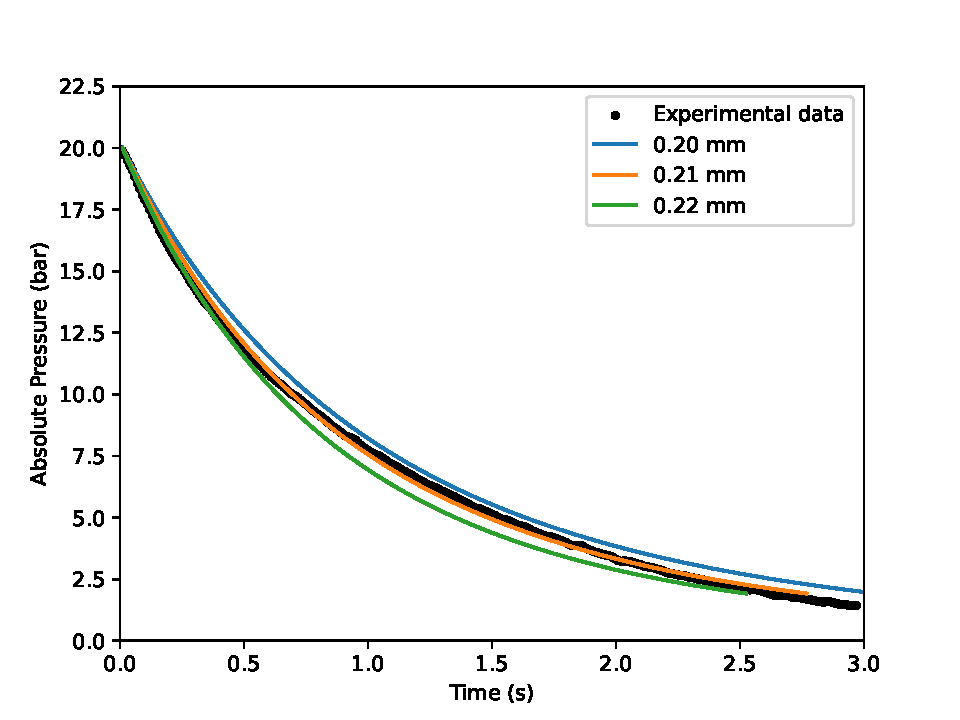
\includegraphics[width=0.75\textwidth]{assets/4 experiments/Saad blowdown fit.pdf}
                \caption{Saad blowdown model and experimental data}
                \label{fig:saad blowdown}
            \end{figure}

            The best match was found to be an area of \qty{3.46e-8}{m^2}, giving a diameter of \qty{0.21}{mm}.

        \subsection{Needle valve effective sonic area $A^*$}

            The WL14H-320P needle valve (see \autoref{fig:Needle valve}) was calibrated to relate its rotation increments to its flow rate. This was undertaken by connecting the valve's input to a gas supply, while the valve's output was connected to a bubble flow meter constructed for this experiment (\autoref{fig:bubble meter}). The bubble flow meter and experiment methodology were presented in \textcite{barigouFluidMechanicsSoap1993}.

            Creating a uniform bubble at the base of the tube, the bubble rises upwards towards the top of the tube as it is displaced by the pressurizing gas. This end of the tube is open to the atmosphere. A stopwatch is started when the bubble passes the base of the green tape line and stopped once the bubble passes the base of the red tape line. These stopwatch measurements are repeated three times and averaged. This enables precise measurement of the volumetric flow rate.

            \begin{figure}[!ht]
                \centering
                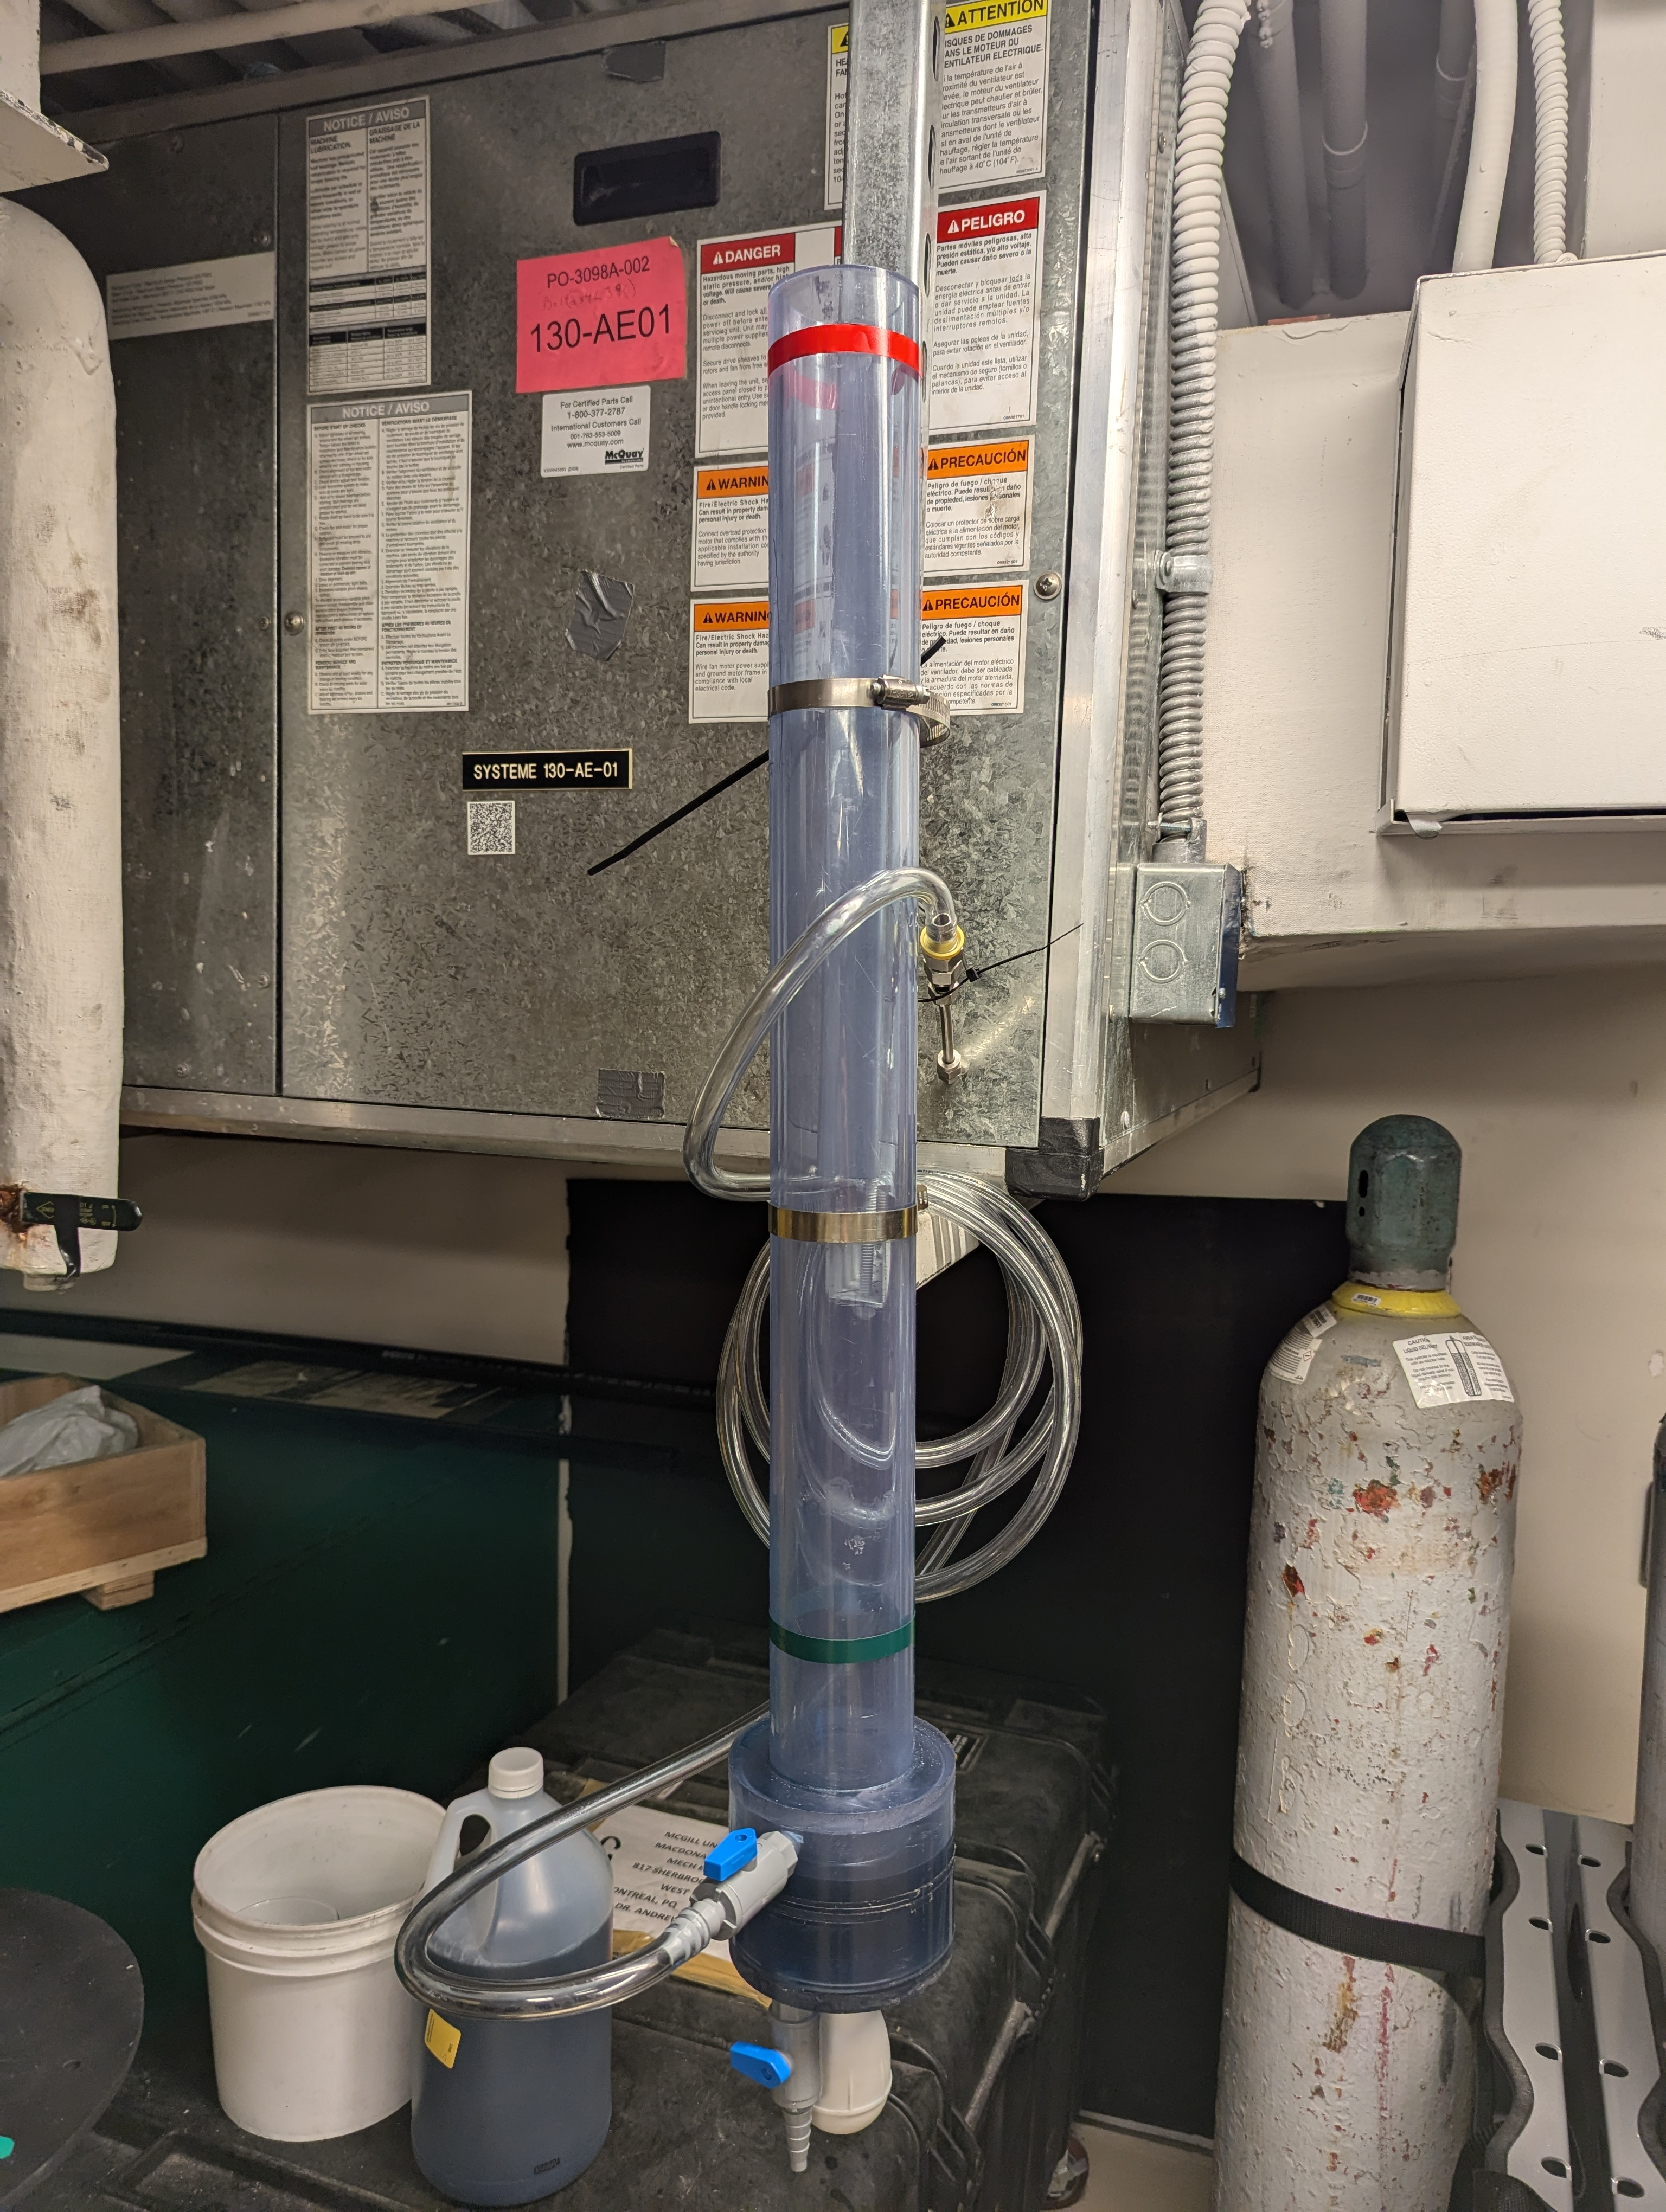
\includegraphics[width=0.5\textwidth]{assets/4 experiments/Bubble meter.png}
                \caption{Bubble meter setup}
                \label{fig:bubble meter}
            \end{figure}

            First, the valve was calibrated with air at \qtylist{3.45;6.89}{bar}. The valve was then calibrated with \qtylist{20;50}{bar} of argon. The volumetric flow rate was measured in both cases for increments of 0.50 rotations to 2.0 rotations.

            The mass flow rate can then be derived by 

            The following calibration results and calculations were taken from \autoref{chp:app Thariq} \todo{right way to cite this?}:

            \begin{table}[!ht]
                \centering
                \caption{Sample of Table 3: Calculated Opening Area for Needle Valve at Different Rotations (Upstream Pressure = 5000 kPa and Outlet Pressure = 100 kPa)}
                \label{tab:opening_area}
                \begin{tabular}{|c|c|c|c|c|}
                \hline
                \textbf{Increment} & \textbf{Volume Flow (L/s)} & \textbf{Mass Flow (g/s)} & \textbf{Area (mm²)} & \textbf{Diameter (mm)} \\ \hline
                0.50 & 0.25 & 0.410 & 0.028 & 0.188 \\ \hline
                1.00 & 0.37 & 0.607 & 0.041 & 0.229 \\ \hline
                1.10 & 0.51 & 0.836 & 0.057 & 0.269 \\ \hline
                1.20 & 0.67 & 1.099 & 0.075 & 0.308 \\ \hline
                1.30 & 0.97 & 1.591 & 0.108 & 0.371 \\ \hline
                1.40 & 1.24 & 2.033 & 0.138 & 0.419 \\ \hline
                \end{tabular}
            \end{table}

            Supposing that the temperature inside V2 during CW LSP thrust tests is \qty{1200}{K} and ... [Other suppositions], \autoref{chp:app Thariq} recommends a rotation increment of approximately 1.33 to produce an $A^*$ of \qty{0.147}{mm^2}. \todo{update with latest}

        \subsection{Summary of results}

            The following table presents a summary of the results determined from cold flow thruster characterisation.

            \begin{table}[!ht]
                \centering
                \caption{Summary of the studied V2 thruster characteristics}
                \label{tab:characteristics}
                \begin{tabularx}{\textwidth}{XX}
                \toprule
                Characteristic                                          &     Value and unit          \\ \midrule
                Needle valve A* under predicted experiment conditions   &     \qty{0.147e-6}{m^2}     \\
                Nozzle A*                                               &     \qty{3.46e-8}{m^2}      \\
                Internal volume of thruster in flowing configuration    &     \qty{9.68e-6}{m^3}      \\
                Average cold flow thrust at 20 bar                      &     \qty{0.96}{N}           \\
                \bottomrule 
                \end{tabularx}
            \end{table}

    \section{Initial QCW LSP thrust tests (hot fire)}
 
            
        Unfortunately, no thrust was measured. NEXT STEP WOULD BE TO TRY CW THRUST TEST, BUT WITH BETTER THRUST STAND CAUSE WE DIDN'T MEASURE ANYTHING WITH 10X THE POWER
            

        



